% This is samplepaper.tex, a sample chapter demonstrating the
% LLNCS macro package for Springer Computer Science proceedings;
% Version 2.21 of 2022/01/12
%
\documentclass[runningheads]{llncs}
%
\usepackage[T1]{fontenc}
% T1 fonts will be used to generate the final print and online PDFs,
% so please use T1 fonts in your manuscript whenever possible.
% Other font encondings may result in incorrect characters.
%
\usepackage{graphicx}
% Used for displaying a sample figure. If possible, figure files should
% be included in EPS format.
%
% If you use the hyperref package, please uncomment the following two lines
% to display URLs in blue roman font according to Springer's eBook style:
%\usepackage{color}
%\renewcommand\UrlFont{\color{blue}\rmfamily}
%\urlstyle{rm}

\usepackage{hyperref}
\usepackage{array}
\usepackage{subcaption}
\usepackage{graphicx}
\usepackage{listings}
% \usepackage{xcolor}
\definecolor{codegreen}{rgb}{0,0.6,0}
\definecolor{codegray}{rgb}{0.5,0.5,0.5}
\definecolor{codepurple}{rgb}{0.58,0,0.82}
\definecolor{backcolour}{rgb}{0.9765,0.9765,0.9765}
\definecolor{identifierColor}{rgb}{0.1835, 0.7812, 0.8086}
\definecolor{keywordColor}{rgb}{0.8594, 0.4023, 0.6641}
\definecolor{stringColor}{rgb}{0.3555, 0.7422, 0.3789}
\definecolor{emphColor}{rgb}{0.8984, 0.7539, 0.3242}

\lstdefinestyle{mystyle}{
    backgroundcolor=\color{backcolour},   
    commentstyle=\color{codegreen},
    keywordstyle=\color{magenta},
    numberstyle=\tiny\color{black},
    stringstyle=\color{stringColor},
    basicstyle=\ttfamily\footnotesize,
    breakatwhitespace=false,         
    breaklines=true,                 
    captionpos=b,                    
    keepspaces=true,                 
    numbers=left,                    
    numbersep=5pt,                  
    showspaces=false,                
    showstringspaces=false,
    showtabs=false,                  
    tabsize=2
}

\lstset{style=mystyle}

\lstdefinelanguage{Kotlin}{
  comment=[l]{//},
  commentstyle={\color{gray}\ttfamily},
  emph={filter, first, firstOrNull, forEach, lazy, map, mapNotNull, println, Class, Throwable, String},
  emphstyle={\color{emphColor}},
  identifierstyle=\color{black},
  morecomment=[s]{/*}{*/},
  morestring=[b]",
  morestring=[s]{"""*}{*"""},
  sensitive=true,
  keywords={!in, !is, abstract, actual, annotation, as, as?, break, by, catch, class, companion, const, constructor, continue, crossinline, data, delegate, do, dynamic, else, enum, expect, external, false, field, file, final, finally, for, fun, get, if, import, in, infix, init, inline, inner, interface, internal, is, lateinit, noinline, null, object, open, operator, out, override, package, private, property, protected, public, receiveris, reified, return, return@, sealed, set, setparam, super, suspend, tailrec, this, throw, true, try, typealias, typeof, val, var, vararg, when, where, while,param},
  keywordstyle={\color{keywordColor}\bfseries},
  stringstyle={\color{stringColor}\ttfamily},
  classoffset=1,
  morekeywords={IXposedHookLoadPackage, XC_LoadPackage, ClipData, CREATOR, newPlainText, getString, getColumnIndex, context, Uri, parse, MethodHookParam, contentResolver, query}, % Library class names
  keywordstyle=[1]\color{cyan},
  classoffset=2,
  morekeywords={@Deprecated, @JvmField, @JvmName, @JvmOverloads, @JvmStatic, @JvmSynthetic, @Throws, Array, Byte, Double, Float, Int, Integer, Iterable, Long, Runnable, Short, Any, Unit, Nothing},
  keywordstyle={\color{gray}\bfseries},
  classoffset=0
}

\usepackage{tikz}
\newcommand*\circled[1]{
    \tikz[baseline=(char.base)]
    {\node[shape=circle,draw,inner sep=1pt] (char) {#1};}
}

\newcommand{\framework}{WhiteLie}

\begin{document}


\title{\framework{}: A Robust System for Spoofing User Data in Android Platforms}
%\titlerunning{A Robust System for Spoofing User Data in Android Platforms}

\author{Anonymous Authors}
% \author{First Author\inst{1}\orcidID{0000-1111-2222-3333} \and
% Second Author\inst{2,3}\orcidID{1111-2222-3333-4444} \and
% Third Author\inst{3}\orcidID{2222--3333-4444-5555}}
% \authorrunning{F. Author et al.}
% % First names are abbreviated in the running head.
% % If there are more than two authors, 'et al.' is used.
% \institute{University1, Location1 \and
% University1, Location2 \\
% \email{email2}\\
% \url{URL2} \and
% University3, Location3\\
% \email{email3}}

\maketitle
\begin{abstract}
    Android employs a permission framework that empowers users to either accept or deny sharing their private data (e.g., location) with an app. However, many apps tend to crash when they are denied permission, leaving users no choice but to allow access to their data in order to use the app. 
    % However, existing approaches either require rooting the device or require recompiling the app. 
    In this paper, we introduce a comprehensive and robust user data spoofing system, \framework{}, that can spoof a variety of user data and feed it to target apps. Unlike prior approaches, \framework{} requires neither device rooting nor altering the app's binary. Through experiments on more than 50 popular Android apps, we demonstrate that \framework{} is able to deceive apps into accepting spoofed data without getting detected. \framework{} does not significantly impact battery consumption, CPU utilization, or the app's execution time. We also show several case studies where \framework{} is useful in protecting user privacy. Our findings underscore the feasibility of implementing user-centric privacy-enhancing mechanisms within the existing Android ecosystem.
    
    \keywords{Android \and User Data Privacy \and Continuous Authentication \and Side-Channel Attacks.}
\end{abstract}
\section{Introduction}
\label{sec:introduction}

Android's open-source nature and vast app ecosystem have contributed to its widespread adoption. For regulating access to sensitive user data, Android employs a permission framework that serves as a gatekeeper~\cite{alkindi2019android}. When using an app, the Android permission framework allows the user to either grant or deny permission for each type of data individually. Unfortunately, the study by Wagner et al.~\cite{ha2013android} reveals that only 17\% of Android users pay attention to permissions while installing/using an app. Once a user grants permission to an app, the permission framework allows unrestricted access to sensitive data endangering the user's privacy~\cite{alkindi2019android}. If the user does pay attention to privacy concerns and denies a permission request, the app often blocks access to not only the features related to the permission but also other features that may not require that permission~\cite{alkindi2019android}. This leaves the user with no alternative but to provide access to their data.

\begin{figure}[t]
    \centering
    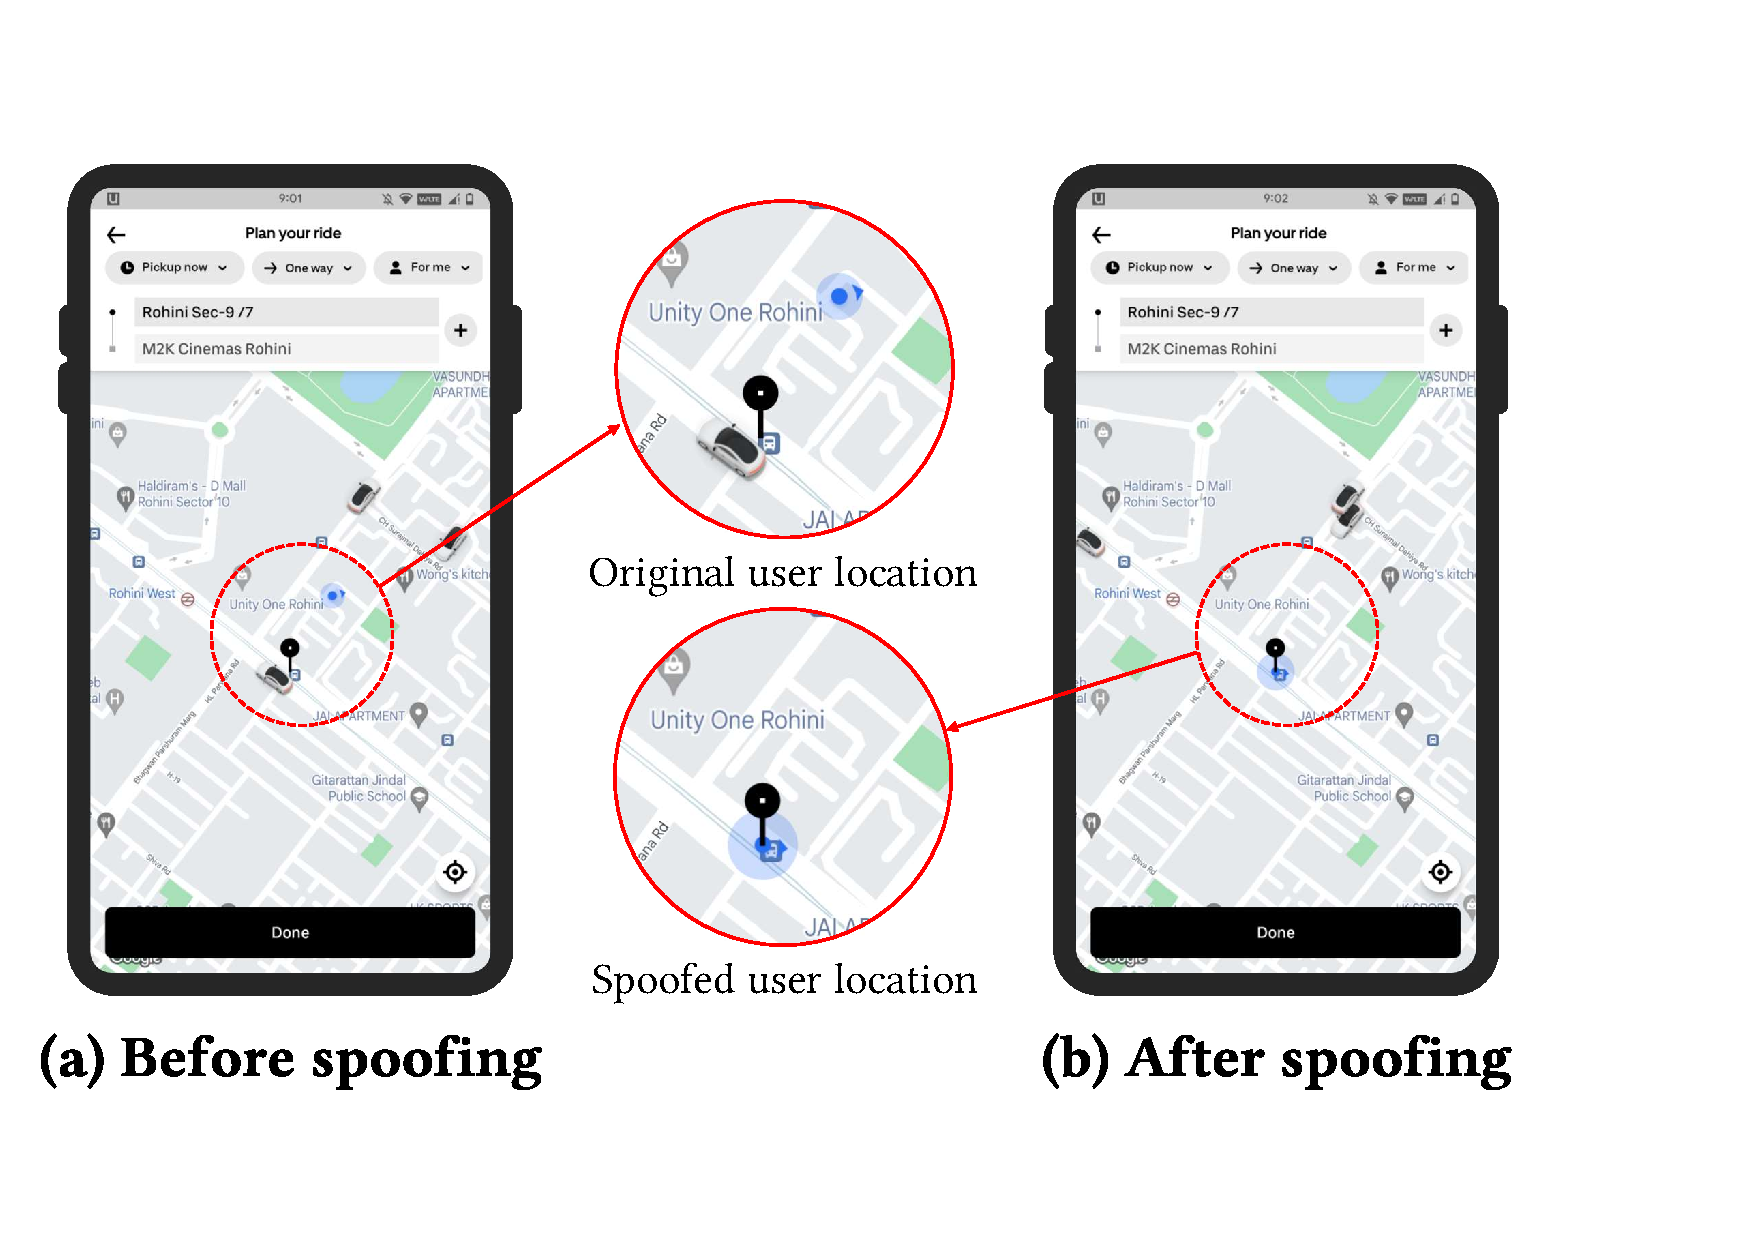
\includegraphics[width=0.75\linewidth]{Figures/Case Studies/uber_screenshots.pdf}
    \caption{Screenshots illustrating how a user can share spoofed location using \framework{} with the Uber app.}
    \label{fig:intro_case_study_uber}
    \vspace{-10pt}
\end{figure}

To enhance user privacy without limiting the app's functionality, users could be equipped with another option: feeding user-controlled, spoofed data to apps. Figure~\ref{fig:intro_case_study_uber} shows such a case study. In Figure~\ref{fig:intro_case_study_uber}a, we observe that even though the user wants to take the cab from the pinned location, Uber encourages the user to share their original location compromising their privacy. Figure~\ref{fig:intro_case_study_uber}b demonstrates how the user can hide their original location and feed the user-specified spoofed location as the current location. This safeguards the user's privacy while still enabling them to utilize Uber's service of finding a cab.

Unfortunately, existing approaches for spoofing the user data involve either modifying the Android OS~\cite{smalley2013security, raval2016you, wu2017context} or rebuilding the target app binary~\cite{backes2015boxify, jeon2012dr}, which have severe limitations in terms of usability and practicality. Modifying the OS requires rooting the device which is not practical for users~\cite{zhang2015android}. Rebuilding app binary is not always successful as it can be easily detected by using Google's Play Integrity API, making the app prevent users from accessing its services~\cite{andPlayIntAPI}. 

To equip users with a practical tool for preserving their privacy, we have built \textit{\framework{}}, a comprehensive and robust user data spoofing system that can spoof any user data fed to an app installed on a typical non-rooted Android device. Our evaluation results indicate that \framework{} robustly spoofs 78.32\% of the requested permissions by 70 popular pre-installed and user-installed Android apps without getting detected by the target apps and without crashing them.

We further show that the deception capability of \framework{} can be utilized to bypass continuous authentication mechanisms. Researchers have been developing a wide range of continuous user authentication mechanisms that rely upon device sensor data (e.g., accelerometer)~\cite{kolokas2019gait, sun2018artificial, thang2012gait, hoang2013adaptive, shih2015flick, nohara2016personal, lu2015safeguard, jain2015exploring, nixon2016slowmo, feng2014tips, abuhamad2020autosen, amini2018deepauth, li2018using, yan2018towards, song2016eyeveri, xia2018motionhacker, hong2016mgra, hong2015waving, miguel2016interaction, zhang2016voicelive, wang2019voicepop, johnson2013secure, khamis2016gazetouchpass, zhu2013sensec, sitova2015hmog, pang2019mineauth, acien2019multilock, zhu2019riskcog, lee2017implicit}. Unlike traditional one-time authentication mechanisms using passwords, a continuous authentication mechanism operates discreetly in the background, constantly monitoring user behavior and biometric features to validate their identity throughout their interaction with an app. Towards that end, to the best of our knowledge, \framework{} is the first system to demonstrate the ineffectiveness of the sensor data-based continuous authentication mechanisms in Android platforms.

\begin{table}
    {\centering
    \begin{tabular} {>{\arraybackslash\centering}m{2.5cm} >{\arraybackslash}m{9.5cm}}
        \hline
         \textbf{Use Case} & \textbf{Example(s)}\\
         \hline
         Bypassing Continuous Authentication & 
         \textbf{MGRA}~\cite{hong2016mgra} (Sec \ref{sec:continuous_authentication_mechanisms}) utilizes the accelerometer data and \textbf{VoiceLive}~\cite{zhang2016voicelive} (Sec \ref{sec:continuous_authentication_mechanisms}) utilizes the smartphone's two different microphones to authenticate users. But \framework{} proves to be capable of bypassing these authentication mechanisms by spoofing the input data. \\
         \hline
         Granting Selective User Data & 
         \textbf{Snapchat}(\hyperref[sec:sc_case_study]{Sec 5.3}) and \textbf{Truecaller}(\hyperref[sec:tc_case_study]{Sec 5.4}) requires users private data like Contacts and Messages to enable users to utilize functionalities provided by them, but this also compromises the private information. However, \framework{} enables users to grant partial data to apps that is essential.\\
         \hline
         Protection from Malicious Apps & 
         \textbf{All Good PDF Scanner} (Sec \ref{sec:malicious_apps}) was granted permissions like Storage and Camera but was detected to be uploading data on the internet in the background, hence its internet access was blocked by \framework{}. \textbf{Unique Keyboard} (Sec \ref{sec:malicious_apps}) was found to be accessing the sensor data while running in the background, therefore \framework{} fed deceived data when app is running in the background.\\
         \hline
         Side-Channel Attack Mitigation & 
         \textbf{Gyrosec}~\cite{lin2019motion} (Sec \ref{sec:side_channel_attack}) records the sensor data while running in the background, and uploads it over the internet. This was mitigated by deceiving the sensor data received by the apps.  \\
         \hline
         Unexpected Sensor Usage Detection & 
         \textbf{Facebook} (Sec \ref{sec:fb_case_study}) requested for Audio permission. But it was found (using \framework{}) to be recording the microphone data when no activity requiring microphone was being used by the user.\\
         \hline
         User Privacy Protection & 
         \textbf{Snapchat} (Sec \ref{sec:sc_case_study}) and \textbf{Truecaller} (Sec \ref{sec:tc_case_study}) provide great features to users but at the cost of sharing private information like Location, Contacts and Messages. \framework{} enables users to enjoy the provided features without compromising private information.\\
         \hline
    \end{tabular}
    }
    \caption{Various use cases of \framework{} and their respective real-world example(s)}
    \label{tab:highlights}
\end{table}

We show that \framework{} proves to be successful in detecting malicious behaviors of and protecting user's private information from malicious apps that have been recently banned by Google. For example, while experimenting with the ``All Good PDF Scanner" Android app, \framework{} detected that the app was uploading user's private files to the internet. \framework{} blocked internet access of the app without crashing or limiting features of the app.

We also demonstrate \framework{}'s potential to detect and mitigate side-channel attacks by malicious apps. For example, our experiments reveal a significant drop in the mobile screen touch position prediction capability of a side-channel attack launched by a malicious app from 81.22\% to just 5.36\% when \framework{} is employed. 

The usage of \framework{} extends beyond protection against malicious apps. We use three real-world apps as case studies to show how \framework{} gives better control over privacy to users. For example, our study of real-world apps uncovers Facebook app recording user's audio while the user is just scrolling over the posts on the home page of Facebook app. This behaviour was not informed to the user by the Android privacy indicator (green dot) but it was detected by \framework{}. \framework{} could spoof audio to protect user's privacy. 

A demonstration video of employing \framework{} for user data spoofing on the Facebook app is available on \href{https://www.youtube.com/watch?v=sXiGUoqFLmk}{Youtube}\footnote{https://www.youtube.com/watch?v=sXiGUoqFLmk}. Table \ref{tab:highlights} highlights various usages of \framework{} with examples.

We validate that spoofing sensitive user data using \framework{} introduces only a minimal average overhead of 2.52\% in battery drain and 5.2 MB of memory during app runs. Each spoofed API call adds an average of 1.64 ms of overhead which did not add any noticeable performance degradation in the apps that we tested.

Overall, we make the following key contributions.

\begin{itemize}
    % [leftmargin=*]
    \item We present \framework{}, a comprehensive and robust system that can be utilized for spoofing any user data fed into an app without rooting the device or modifying the app's source code. We show that \framework{} adds minimal overhead.
    \item The inherent design of \framework{} enables it to bypass continuous authentication mechanisms shedding light on the limitations and weaknesses present in the current implementation of these mechanisms. 
    \item We show how \framework{} mitigates direct privacy attacks and side-channel attacks by malicious apps.
    \item We demonstrate how \framework{} can protect user privacy on real-world apps such as Facebook, Snapchat, Truecaller, and Uber. 
\end{itemize}

The rest of the paper is organized as follows. Section~\ref{sec:motivation} presents the motivation for developing a system to spoof user data. Section~\ref{sec:methodology} explains the methodology employed in \framework{} to spoof user data accessed by target apps. Section~\ref{sec:architecture} presents the detailed architecture of \framework{}. Sections~\ref{sec:mitigating_sca} and \ref{sec:protecting_up} showcase usefulness of \framework{}. Section~\ref{sec:mitigating_sca} shows how \framework{} can detect and mitigate privacy attacks from malicious apps to protect user privacy. Section~\ref{sec:protecting_up} shows how \framework{} empowers users to get better control over their privacy while using bening real-world apps. Section~\ref{sec:results} provides the evaluation results on the overhead of \framework{}. Section~\ref{sec:related_work} presents an overview of prior approaches. We conclude the paper in Section~\ref{sec:conclusion}.
\section{Motivation for Spoofing User Data}
\label{sec:motivation}

The motivation for our work stems from the realization that current approaches for protecting user data in the Android ecosystem are insufficient leaving user data exposed to privacy violations from the installed apps. 

\subsection{Inadequate Android Permission Framework}

The Android platform provides a permission framework that enables the user to control the data access privileges granted to individual apps. It aims to safeguard sensitive user data by restricting unauthorized access. However, it has been found to be inadequate failing to prevent apps from collecting sensitive data. Researchers~\cite{hasan2013sensing, simon2013pin, ba2020learning, shen2015input, lin2019motion} have shown that non-runtime permissions, also referred to as ``normal permissions'', like those related to the inertial measurement unit, can contain sensitive information, but the Android permission framework grants access to them without notifying the user.

For runtime permissions, also referred to as ``dangerous permissions'', like location, requested by apps, the user is presented with a binary choice to either grant or deny each permission. Granting a requested permission can result in a privacy breach while denying it triggers a \texttt{SecurityException} in the app. If the exception is not handled properly, the app crashes. Even if the exception is handled correctly, due to a lack of permission, the app limits its services. Further, Wagner et al.\cite{wijesekera2017feasibility} noted that only 17\% of users pay attention to permissions during installation. Recently added options, such as ``\textit{Only this time}'' and ``\textit{While using the app}'', in the permission framework aim to protect user privacy by preventing background permission usage. Hence, the existing permission framework lacks flexibility, leaving users with limited choices.

\subsection{Limitations of Existing User Data Spoofing Mechanisms}

The aforementioned inadequacy of the Android permission framework has motivated researchers to look for an alternative option, i.e., to deceive the user data fed to the apps. While modifying the source code of the Android OS or target apps~\cite{backes2015boxify, jeon2012dr, raval2016you, smalley2013security, wu2017context} might seem like a solution, this approach necessitates the creation of a custom ROM. However, installing custom ROMs on Android devices requires root privileges, making it impractical for most users. Additionally, modifying the source code of each target app is not a scalable solution. This mechanism can also be easily detected if Google's Play Integrity API is utilized in the target app~\cite{andPlayIntAPI}.

\begin{table}[h]
    {\centering
    \begin{tabular}{>{\centering\arraybackslash}m{2.5cm} > {\centering\arraybackslash}m{3cm} >{\centering\arraybackslash}m{4cm} >{\centering\arraybackslash}m{2.5cm}}
        \hline
          \textbf{Modality} & \textbf{Framework} & \textbf{User Data} & \textbf{Accuracy} \\
         \hline
         \textbf{Gait} \\
         & ~\cite{kolokas2019gait, sun2018artificial, thang2012gait, hoang2013adaptive} & Ac, Ca, Gy, Mg & 91-95\% \\
         \hline
         
         \textbf{Gesture} \\
         Flick & ~\cite{shih2015flick, nohara2016personal} & Ac, Gy & 92.8-98\% \\
         
         Swipe & ~\cite{lu2015safeguard, jain2015exploring} & Ac, Or, To \\
         
         Touch & ~\cite{nixon2016slowmo, feng2014tips} & To & 89\%\\
         \hline

         \textbf{Motion} \\
         Free & ~\cite{abuhamad2020autosen, amini2018deepauth, li2018using} & Ac, Gy, Mg & 96.7-97.5\% \\
         
         Shake & ~\cite{yan2018towards} & Ac, Gy & 96.87\%\\

         Eye & ~\cite{song2016eyeveri} & Ca & 88.73\% \\

         IaH & ~\cite{xia2018motionhacker} & Ac, Gy & 32.8\% \\
         
         Gesture & ~\cite{hong2016mgra, hong2015waving} & Ac & 92.2-95.8\%\\

         \hline

         
         
         \textbf{Voice} \\
         & ~\cite{miguel2016interaction, zhang2016voicelive, wang2019voicepop, johnson2013secure} & Mi & 93.5-99.3\% \\
         \hline 
        
         \textbf{Multimodal} \\
         Ge, Mo & ~\cite{khamis2016gazetouchpass, zhu2013sensec} & Ac, Gy, Or, To & 65\% \\
         
         Ga, Ge, Mo & ~\cite{sitova2015hmog} & Ac, Gy, To & \\

         Be, Ga, Ge & ~\cite{pang2019mineauth, acien2019multilock} & Ac, Nw, Tk, To & 85-97.1\% \\
         
         Ga, Ge & ~\cite{zhu2019riskcog, lee2017implicit} & Ac, Gy, Li, Mg & 95.6-98.1\% \\

        \hline
        \multicolumn{4}{p{12cm}}{\footnotesize \textbf{Ac}: Accelerometer, \textbf{Ca}: Camera,  \textbf{Gr}: Gravity Sensor, \textbf{Gy}: Gyroscope, \textbf{Li}: Light Sensor, \textbf{Mg}: Magnetometer,  \textbf{Mi}: Microphone, \textbf{Nw}: Network, \textbf{Or}: Orientation, \textbf{To}: Touch, \textbf{Tr}: Tracking} \\
        \hline
        
        \multicolumn{4}{p{12cm}}{\footnotesize \textbf{Be}: Behaviour, \textbf{Ga}: Gait, \textbf{Ge}: Gesture, \textbf{IaH}: In-air Handwriting, \textbf{Mo}: Motion}\\
        \hline
    \end{tabular}
    }
    \caption{Existing continuous authentication methods.}
    \label{tab:ca_approaches_deceivable}
\end{table}

\subsection{Spoofing: Achilles Heel of Continuous User Authentication}
\label{sec:continuous_authentication_mechanisms}

The conventional knowledge-based authentication approaches require a user to provide information like passwords to access their device. While these methods are simple to implement, they suffer from drawbacks such as the need for frequent re-entering and the possibility of reuse by an attacker. To mitigate these limitations, continuous authentication mechanisms have been implemented that verify the user's identity based on their behavioral biometrics such as keystroke dynamics, touch gestures, motion, and voice. By leveraging such inherent biometric signatures of the user, this approach aims to prevent unauthorized access. Table \ref{tab:ca_approaches_deceivable} offers an overview of different continuous authentication mechanisms across five widely used modalities. 

The user's biometric signatures are captured implicitly through various data streams, including interaction, environmental information, and sensory data. Hence, the underlying assumption to justify the security of these mechanisms is that these biometric signatures are unique to the user and difficult for attackers to replicate. Upon analyzing these approaches, we determined that the majority of them rely on user data (specifically, sensor data) as the primary data source for user authentication. Hence, these authentication mechanisms can be bypassed by manipulating the user data (especially sensor data) fed into them. The attacker can simply present false sensor data replicating the data recorded when the authentic user was utilizing the device. This can lead the authentication mechanism to erroneously conclude that the genuine user is using the device and allow the attacker to gain unauthorized access to sensitive data or perform actions on behalf of the legitimate user. 

However, we note that since there is no robust mechanism for spoofing the user data in the existing literature, the aforementioned attack on the continuous authentication mechanisms is difficult to realize in the real world. The absence of such a strong attack has resulted in the wide acceptance of weak continuous authentication methods~\cite{kolokas2019gait, sun2018artificial, thang2012gait, hoang2013adaptive, shih2015flick, nohara2016personal, lu2015safeguard, jain2015exploring, nixon2016slowmo, feng2014tips, abuhamad2020autosen, amini2018deepauth, li2018using, yan2018towards, song2016eyeveri, xia2018motionhacker, hong2016mgra, hong2015waving, miguel2016interaction, zhang2016voicelive, wang2019voicepop, johnson2013secure, khamis2016gazetouchpass, zhu2013sensec, sitova2015hmog, pang2019mineauth, acien2019multilock, zhu2019riskcog, lee2017implicit}.

To mitigate the insufficiency of the Android permission framework and to establish a practical benchmark for continuous authentication mechanisms, there is a need for a more robust and comprehensive approach to spoof user data in the Android ecosystem. This paper aims to address this critical gap by identifying and addressing the limitations of existing data spoofing mechanisms.
\newpage
\section{\framework{} Methodology}
\label{sec:methodology}

We now provide the methodology to achieve the goal of deceiving user data fed to the apps without rooting the device or altering the source of the apps.

\subsection{Background on Hooking}
In Android, a typical user does not have permission to modify the apps or OS behaviour. However, \textit{hooking} into OS and apps is one of the most practical options to alter the behaviour of an app. Hooking is a technique of code modification that changes the behaviour of the original code running sequence by inserting instructions into the code segment. 

Hooking can be performed in two ways: statically and dynamically. The static hooking technique injects hooks before app execution by altering the byte code of the app or by injecting custom shared libraries. However, static hooking causes permanent alteration and can be detected by an app using a digital signature. 

Dynamic hooking technique applies ``hooks'' at runtime by modifying the code stored in volatile memory (temporary modification), allowing hooking decisions based on the runtime environment. Android's Dalvik VM utilizes Dynamic Linkers' ``virtual method table'' to jump to the memory location on a method call, hence \textit{Call Diversion} can be employed to inject hooks in the hooked method lookup table entry. 

\begin{figure}[t]
    \centering
    \begin{subfigure}{0.48\linewidth}
        \vspace{7mm}
        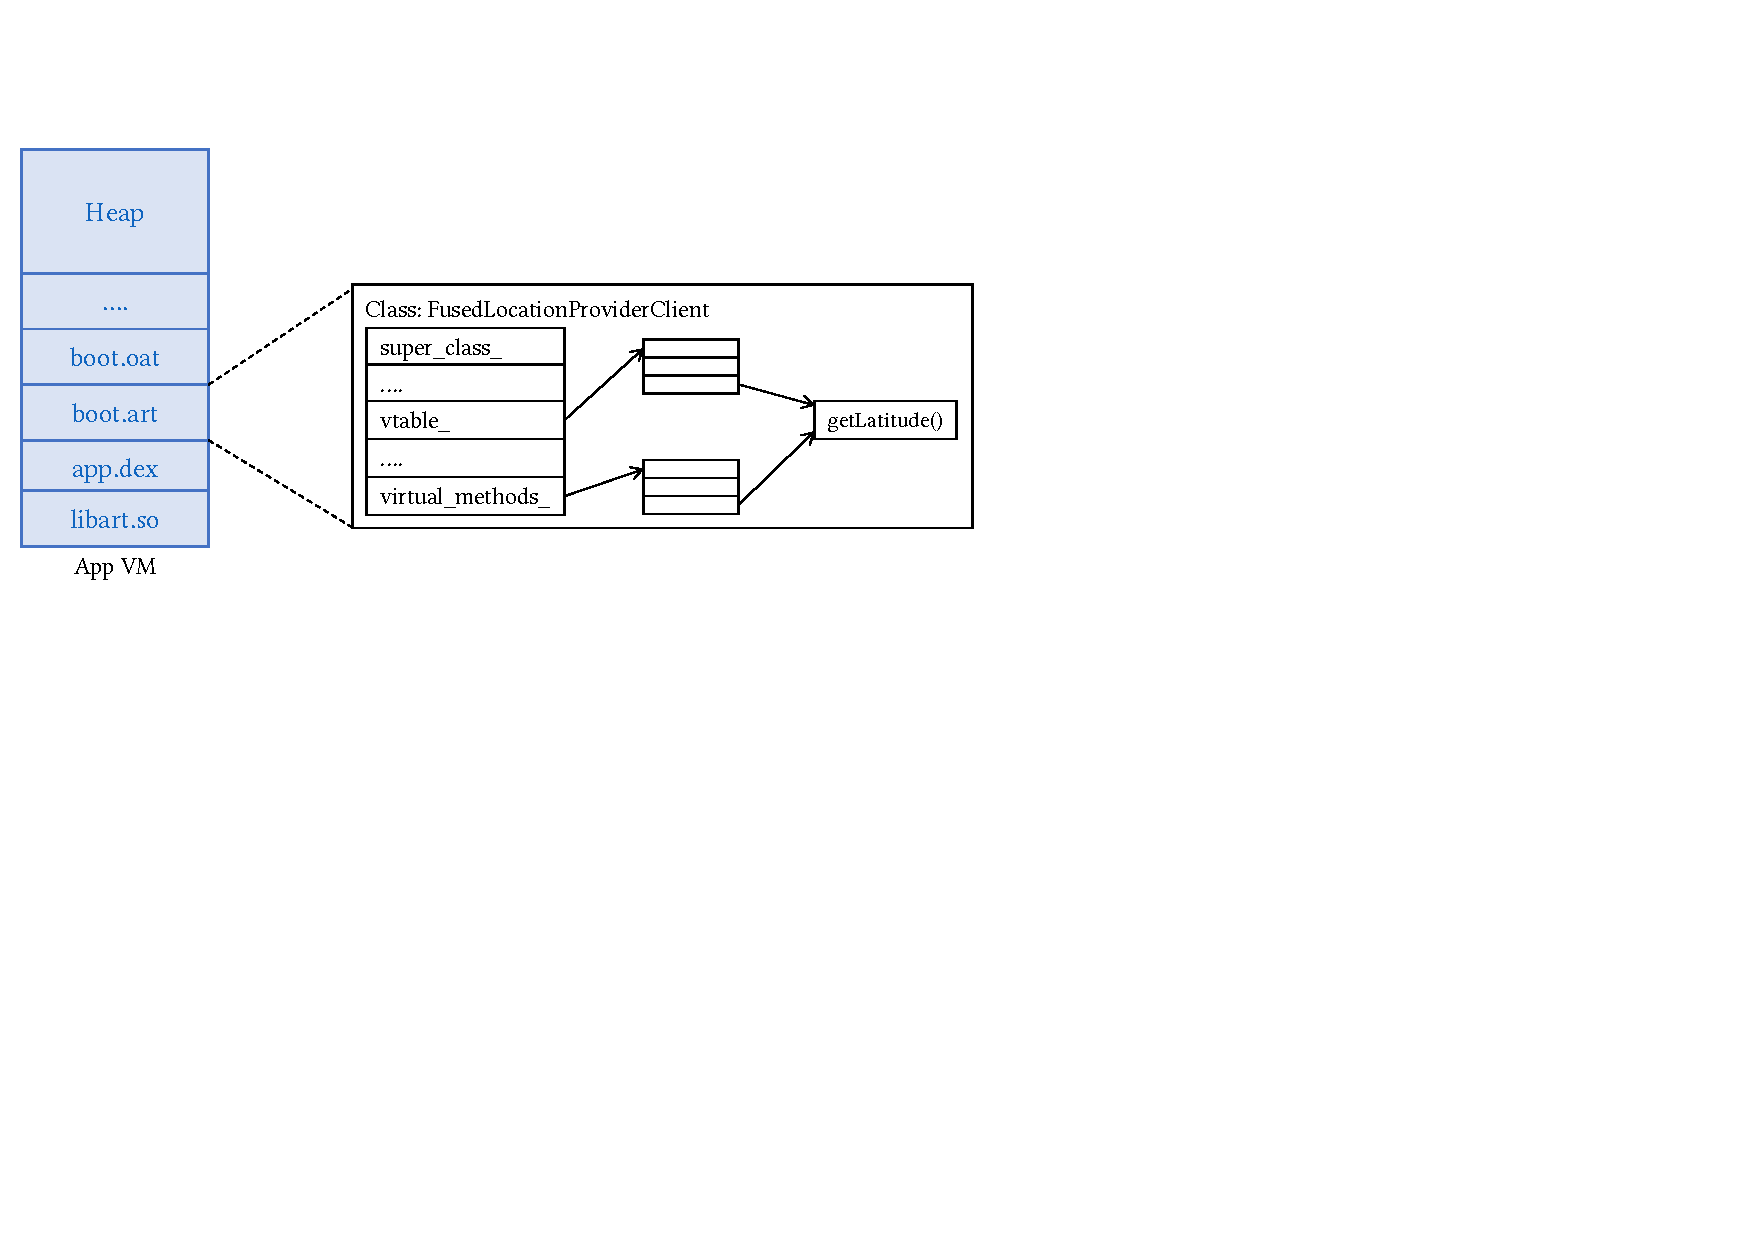
\includegraphics[width=\linewidth]{Figures/Background/virtual_memory_without_deceiver.pdf}
        \caption{Original method call.}
        \label{fig:vrtulMemMthdCall_woFr}
    \end{subfigure}
    \begin{subfigure}{0.48\linewidth}
        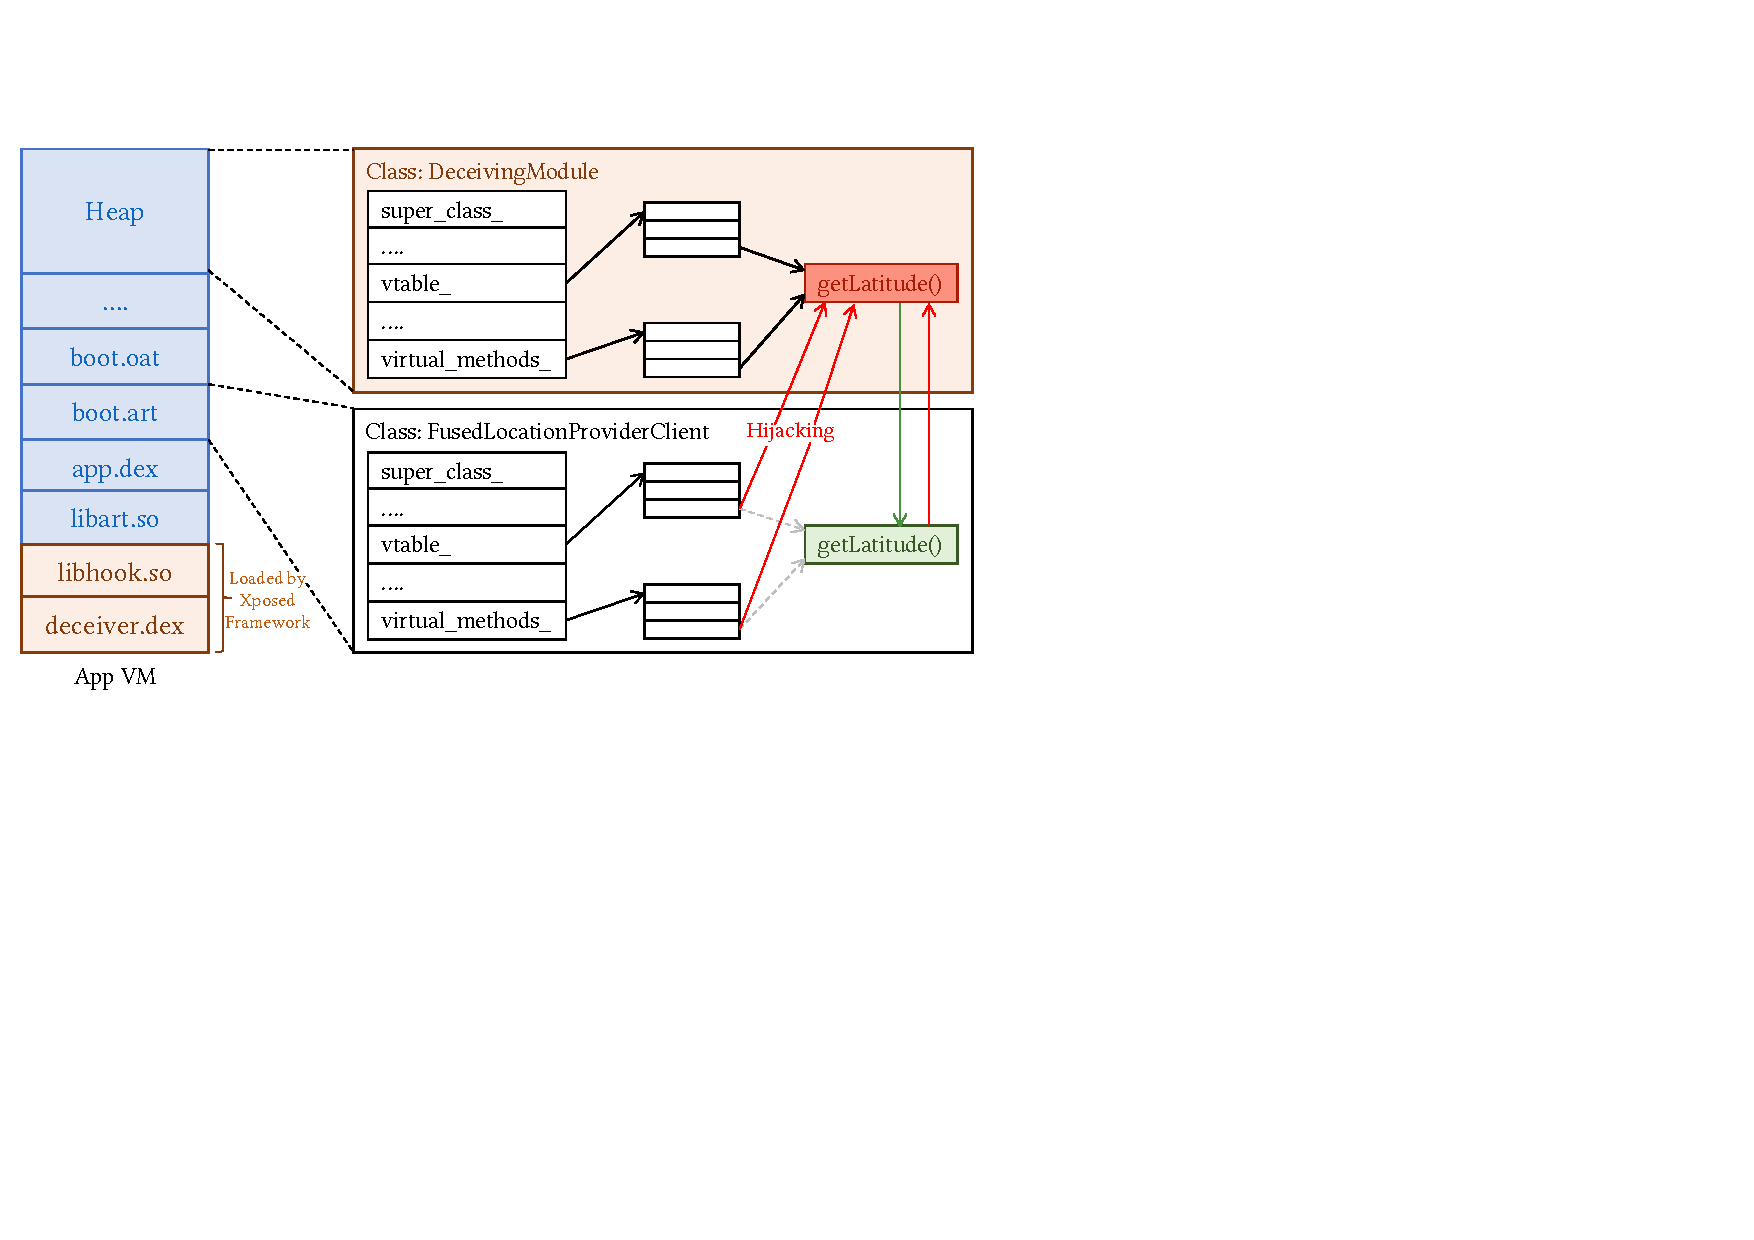
\includegraphics[width=\linewidth]{Figures/Background/virtual_memory_with_deceiver.pdf}
        \caption{Method call with \framework{}.}
        \label{fig:vrtulMemMthdCall_wFr}
    \end{subfigure}
    \caption{Example illustrating how the Xposed module class method hijacks the original method call.}
    \label{fig:vrtulMemMthdCall}
\end{figure}

In Figure \ref{fig:vrtulMemMthdCall}, we present an overview of dynamic hooking in Android using the \texttt{Location.getLatitude()} method. Figure \ref{fig:vrtulMemMthdCall_woFr} illustrates the conventional process of method call jumps. The virtual memory of the target app encompasses the heap space and various files loaded by the \textit{Zygote} process to initiate the app process. Zygote is a process started by the Android Framework during the OS boot. It is a template process preloaded with Java-shared libraries in memory, responsible for launching apps and services. 

The \texttt{boot.oat} and \texttt{boot.art} files serve as boot images to speed up the boot proces containing frequently used class source code and the pre-initialized heap respectively. The heap of the target class is stored in the \texttt{boot.art} file. The Dalvik Executable code of the app and the shared libraries are stored in the \texttt{app.dex} and \texttt{libart.so} respectively. When the target method is invoked by the app, the existence of the target class is checked in the \texttt{boot.art} file. If the class is found, the addresses of the target methods are determined using the virtual tables stored in the heap. Consequently, the execution jumps to the identified address.

% In contrast, 
Figure \ref{fig:vrtulMemMthdCall_wFr} depicts the process of hooking. The hooked application's virtual memory is loaded with the \texttt{libhook.so} shared library by the hooking module, facilitating the hooking operations. Subsequently, the hooks defined by the hooking app (\texttt{hook.dex}) are loaded by the hooking module as Dalvik Executables (same as app code). Upon completion, \texttt{libhook.so} intervenes and loads the hooking classes into the app's heap space, modifying the entries of the target class virtual tables with the addresses of the hooking class methods. Consequently, when the app calls the hooked methods, the calls are redirected to the hooking class methods instead of the original methods. Finally, the original method is invoked by storing its address at the end of the hooking method.

% \begin{lstlisting}[caption={Kotlin code to deceive Clipboard permission data with the data defined by user in \textit{Deceit} policies.},label={lst:clipboardDeceiver},language=Kotlin,float=*]
class SpoofingModule: IXposedHookLoadPackage {
    companion object {
        fun getClass(clsName: String): Class<*> = Class.forName(clsName, false, lpparam.classLoader)    
    }
    
    @Throws(Throwable::class)
    override fun handleLoadPackage(lpparam: XC_LoadPackage.LoadPackageParam) {
        hookAllMethods(getClass(ClipData.CREATOR.javaClass.name), "createFromParcel", XC_MethodHook() {
            @Throws(Throwable::class)
            override fun beforeHookedMethod(param: MethodHookParam) {
                val uri = Uri.parse("content://com.xposedModule.provider/deceitSettings")
                val cursor = context.contentResolver.query(uri, null, null, null, null) ?: return
                val blockClipboard = cursor.getInt(cursor.getColumnIndex("blockClipboard")
                cursor.close()
                if(blockClipboard) param.result = null
            }

            @Throws(Throwable::class)
            override fun afterHookedMethod(param: MethodHookParam) {
                param.result ?: return
                val uri = Uri.parse("content://com.xposedModule.provider/deceits")
                val cursor = context.contentResolver.query(uri, null, null, null, null) ?: return
                val clipboardLabel = cursor.getString(getColumnIndex("clipboardLabel")) ?: "dummyLabel"
                val clipboardText = cursor.getString(getColumnIndex("clipboardText")) ?: "dummyText"  
                cursor.close()
                param.result = ClipData.newPlainText(clipboardLabel, clipboardText)
            }       
        })   
    }
}
\end{lstlisting}

\subsection{Hooking on Non-Rooted Device}

We found that the most suitable solution to deceive user data is app hooking. However, on non-rooted devices, users are restricted from accessing the root and hooking various processes within the system. To gain hooking capabilities, root access to the \textit{Zygote} process is required. 

For this, we utilize \textit{adb} (\textit{Android Debug Bridge}), a command-line tool typically utilised for debugging apps, but also capable of controlling Android devices and executing shell commands. \textit{adb} provides user-installed apps with privileged access to the system APIs. This access is limited till the device is in an active connection with the \textit{adb} tool. This limitation is futher tackled by the Shizuku service by exploiting \textit{adb} shell access. Shizuku provides privileged access to system APIs to user-installed apps by running a dedicated process with shell-level permissions, acting as a proxy between the apps and the OS. This level of access is sufficient for hooking the target apps to spoof the user data. 
%The users need to restart the Shizuku service after every device reboot. 

Employing the Shizuku service, we use LSPatch, an Xposed framework for non-rooted devices, for hooking the target apps by injecting the hooks into app processes. This allows users to define the required app behaviour within the Xposed module to make the target app execute their desired actions. Both the Shizuku service and LSPatch are open-source and user-controlled, they only grant root privileges to the modules and apps chosen by the user, ensuring that the attack surface remains unchanged.

\subsection{Spoofing User Data with Hooking}

In Listing \ref{lst:clipboardDeceiver}, we present the approach employed to spoof the Clipboard data with custom spoofed data by hooking. Typically, the app retrieves clipboard data by calling the \texttt{ClipboardManager.getPrimaryClip()} method. However, to modify the result of this method, multiple other methods need to be hooked. Alternatively, a more efficient approach involves hooking \texttt{ClipData.CREATOR.createFromParcel()} method, as ultimately, this method is called by the former method to return the clipboard data. To hook this method, we utilise Xposed's \texttt{handleLoadPackage()} in Line~7.

Using this mechanism, the Clipboard data can either be blocked or modified before feeding into the target apps. In the before hook, Line 11-15 lists the code for blocking the clipboard data from feeding into the target apps. Using \textit{ContentProvider} the Xposed module is gathering the user's choice on blocking the clipboard data in Line 11-13. And then in Line 15, if the user opts for blocking the clipboard data, then the resultant part of the function call is updated with null object. This blocks the original method call and execution returns back to the method from where the call for the hooked method is made. 

Similarly, in the after hook, i.e. Lines 20-26, the clipboard data is deceived as plain text data as per the user policy. The user-defined deceived data is fetched from the \textit{ContentProvider} in Line 21-24. And then in Line 26, the result of the method call is updated with a new \texttt{ClipData} object initialised with fetched deceived result.

\framework{} offers diverse policies for deceiving various permissions. For instance, one policy for spoofing camera permission involves blurring the image when the app is operating in the background. In this scenario, \framework{} utilizes the \texttt{ActivityManager} to determine whether the target app is running in the background or not. If it is found to be running in the background while accessing the camera permission, \framework{} blurs the frames supplied to the app by manipulating the pixels. Another intriguing policy employed by \framework{} involves providing a noise audio fed if an app unnecessarily requests Audio permission.

\subsection{\framework{} and its Robustness}
In this section, we present \framework{}'s mechanism to achieve the functionality of spoofing the user data fed into other apps and discuss its performance against real-world apps highlighting its robust nature.

\mysubsubsection{Robust Mechanism} 
By utilising dynamic hooking, \framework{} effectively manipulates user data in other apps by modifying the source code stored in volatile memory, thus avoiding permanent alterations on disk. As a result, the injected hooks cannot be detected using APK signatures or Google's Play Integrity API, making \framework{} resilient against these security measures. Moreover, \framework{} follows a methodology of spoofing user data instead of outright revoking permissions based on context. This approach ensures that \framework{} remains crash-proof, providing a reliable and robust solution.

\mysubsubsection{Spoofing Real-world Apps}
The capability of \framework{} against real-world apps in protecting user privacy by spoofing was explored using 50 real-world apps downloaded from the Google Play Store, and 20 pre-installed Android apps. All permissions requested by the apps were granted beforehand, and the apps were subjected to 20 minutes of manual usage. All experiments were conducted on a \textit{Samsung Galaxy M21} smartphone with a 2.3 GHz octa-core processor and 4 GB of RAM running Android 12. The outcomes were documented for each permission, taking into account visual confirmation of spoofed user data and the logs captured by \framework{}.

The heatmap depicted in Figure \ref{fig:intro_heatmap} provides an overview of the \framework{}'s performance when applied to the most popular apps on the Google Play Store. The dark green region of the heatmap signifies the successful deception of permissions for corresponding Android apps. The light green, orange, and red regions indicate permissions that were not requested, not utilized, and could not be deceived, respectively. 
% 531, 147, 41, 678, 73.85% -> 78.32%, 20.44 -> 21.68%

Out of the 678 permissions requested by 70 apps, the \framework{} achieved a \textbf{78.32\%} success rate in spoofing user data. We could not ascertain the deception for 21.68\% of the permissions because although they were granted to the app, they were not explicitly requested during the experiments. These encouraging results demonstrate the robustness of the \framework{}'s mechanism and design in real-world scenarios as none of the apps crashed and functioned as expected.

\begin{figure}[t]
    \centering
    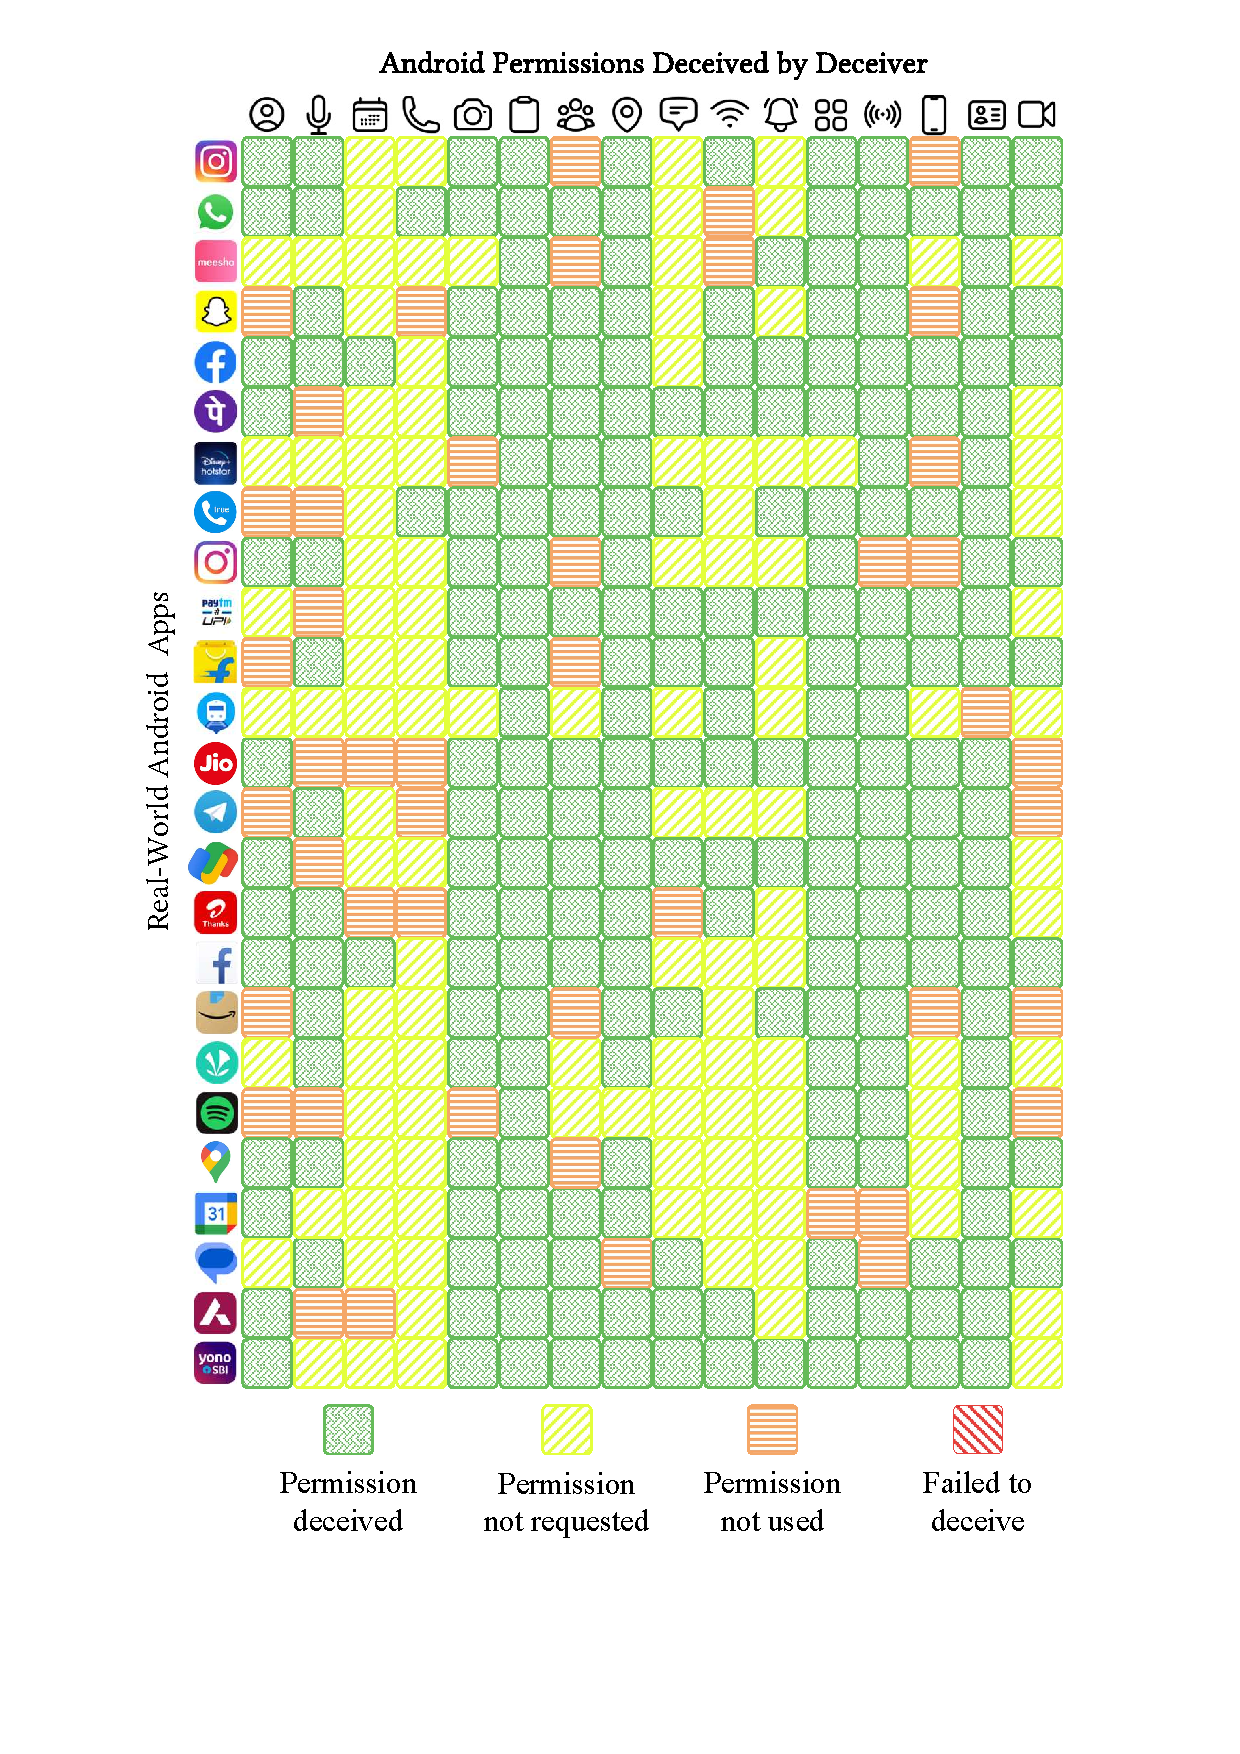
\includegraphics[width=0.6\linewidth]{Figures/Introduction/heatmap.pdf}
    \caption{Heatmap illustrating status of user data deceived for various popular apps by \framework{}.}
    \label{fig:intro_heatmap}
\end{figure}

\mysubsubsection{Hooking Hidden APIs} 
Certain permissions such as sensors, involve method calls returning instances of \textit{Android Non-SDK Interfaces} classes also known as \textit{Hidden APIs} like \texttt{InputSensorInfo}. Accessing these Hidden APIs is restricted for \textit{JNI} and \textit{Java Reflections}. \framework{}'s hooks corresponding to Hidden APIs bypass these restrictions and instantiate classes with deceived data using the \textit{LSPlant}. Out of 78.32\% successfully deceived user data, 23.16\% were deceived by hooking hidden APIs.

\mysubsubsection{Isolation} \framework{} requests the \textit{Query All Packages} permission to facilitate and simplify its privacy protection functionalities which is a non-runtime (normal) permission and the only permission requested by \framework{}. Notably, \framework{} operates offline, severing any external connections and isolating itself from the internet, establishing a secure and trustworthy environment.

\section{Implementation}
\label{sec:architecture}
\newpage
\section{Privacy Protection against Real-World Apps}
\label{sec:protecting_up}


In Figure~\ref{fig:intro_case_study_uber}, we showed how \framework{} can be effectively used to protect user privacy while they are using Uber. In this section, we use three more real-world Android apps to showcase privacy advantages of \framework{}.

\subsection{com.katana.facebook (v404.0.0.35.70)}
\label{sec:fb_case_study}
 
During the experiment, while scrolling through posts in the Facebook app's \textit{Home} activity and without engaging any other app features, \framework{}'s \textit{Resource Access Log Reporter} recorded instances of the Facebook app accessing audio permission as shown in Figure~\ref{fig:case-study-facebook}(a). On further investigation, we found that the Facebook app was using \texttt{MediaRecorder} to access the device microphone. Moreover, the Android's privacy indicator~\cite{andPrivacyIndicator} (green dot), which indicates active use of the device microphone, did not appear when \framework{} logged the use of audio permission. We found this surprising.

We were able to repeat this behavior with a custom mobile app i.e. we used \texttt{MediaRecorder} API to successfully record audio while Android's privacy indicator did not show up. We believe it is a bug in Android's privacy indicator implementation. We have reported this to Android and plan to open source this custom app responsibly.

Hence, \framework{} was able to detect microphone usage that was not indicated by Android. Moreover, \framework{} successfully spoofed audio data requested by the Facebook app. 

Similar to the unexpected microphone access, \framework{} also logged instances of calendar data access by the Facebook app while searching for nearby events. The app reads user's calendar events to display their availability when the user is viewing nearby events. Users can configure \framework{} to manipulate calendar data in a way that allows the Facebook app to receive information about their availability without compromising sensitive details about individual events. This involves spoofing fields like event name and location. \framework{} could spoof the app's request for calendar data by providing a list of manipulated events.

\begin{figure}[t]
    \centering
    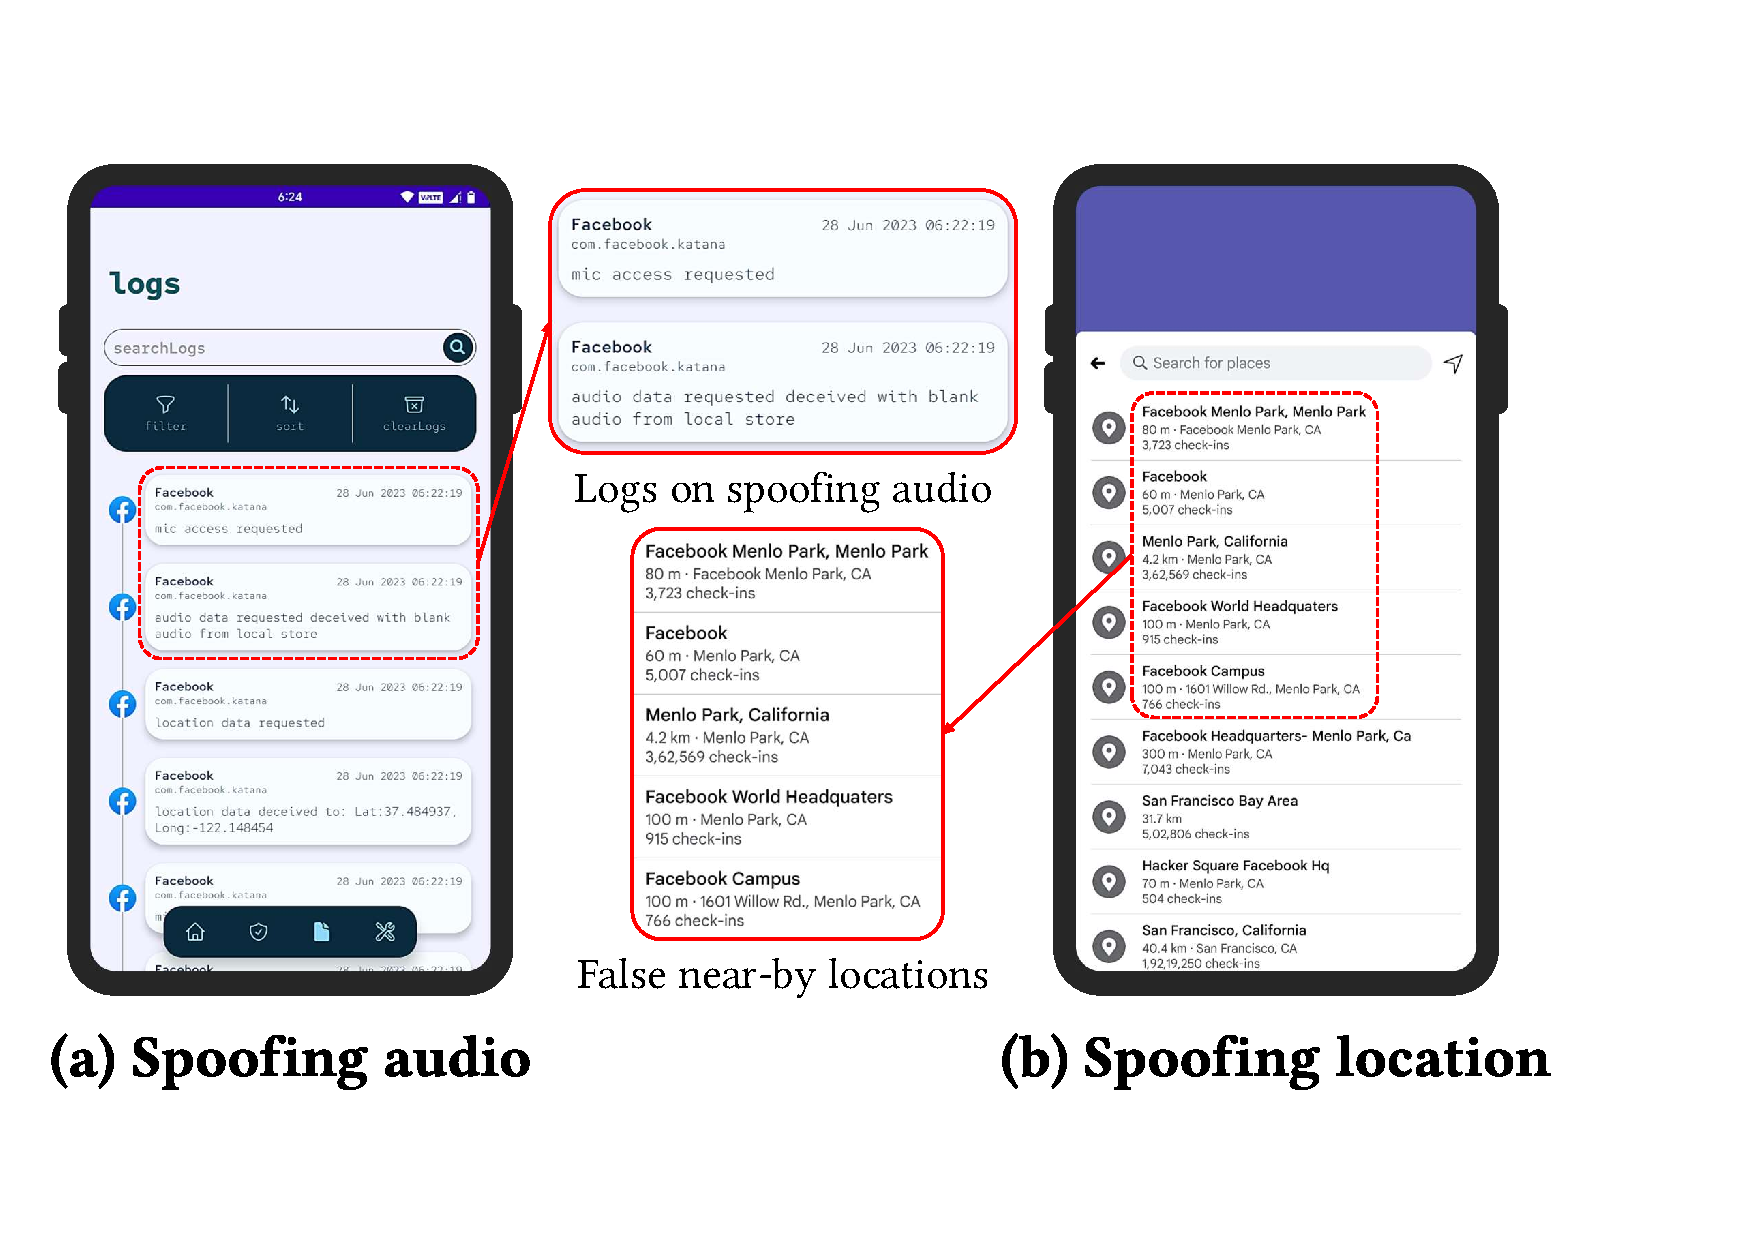
\includegraphics[width=0.75\linewidth]{Figures/Case Studies/facebook_screenshots.pdf}
    \caption{Screenshots demonstrating deceiving location and audio data using \framework{} for the Facebook app.}
    \label{fig:case-study-facebook}
\end{figure}

Nearby events were listed using user's location data. As shown in Figure~\ref{fig:case-study-facebook}(b), we could effectively spoof the fine-grained GPS location data with a nearby location ensuring that the reported nearby places and events were same without compromising user's exact location. 

\subsection{com.snapchat.android (v12.24.0.34)}
\label{sec:sc_case_study}

\begin{figure}[t]
    \centering
    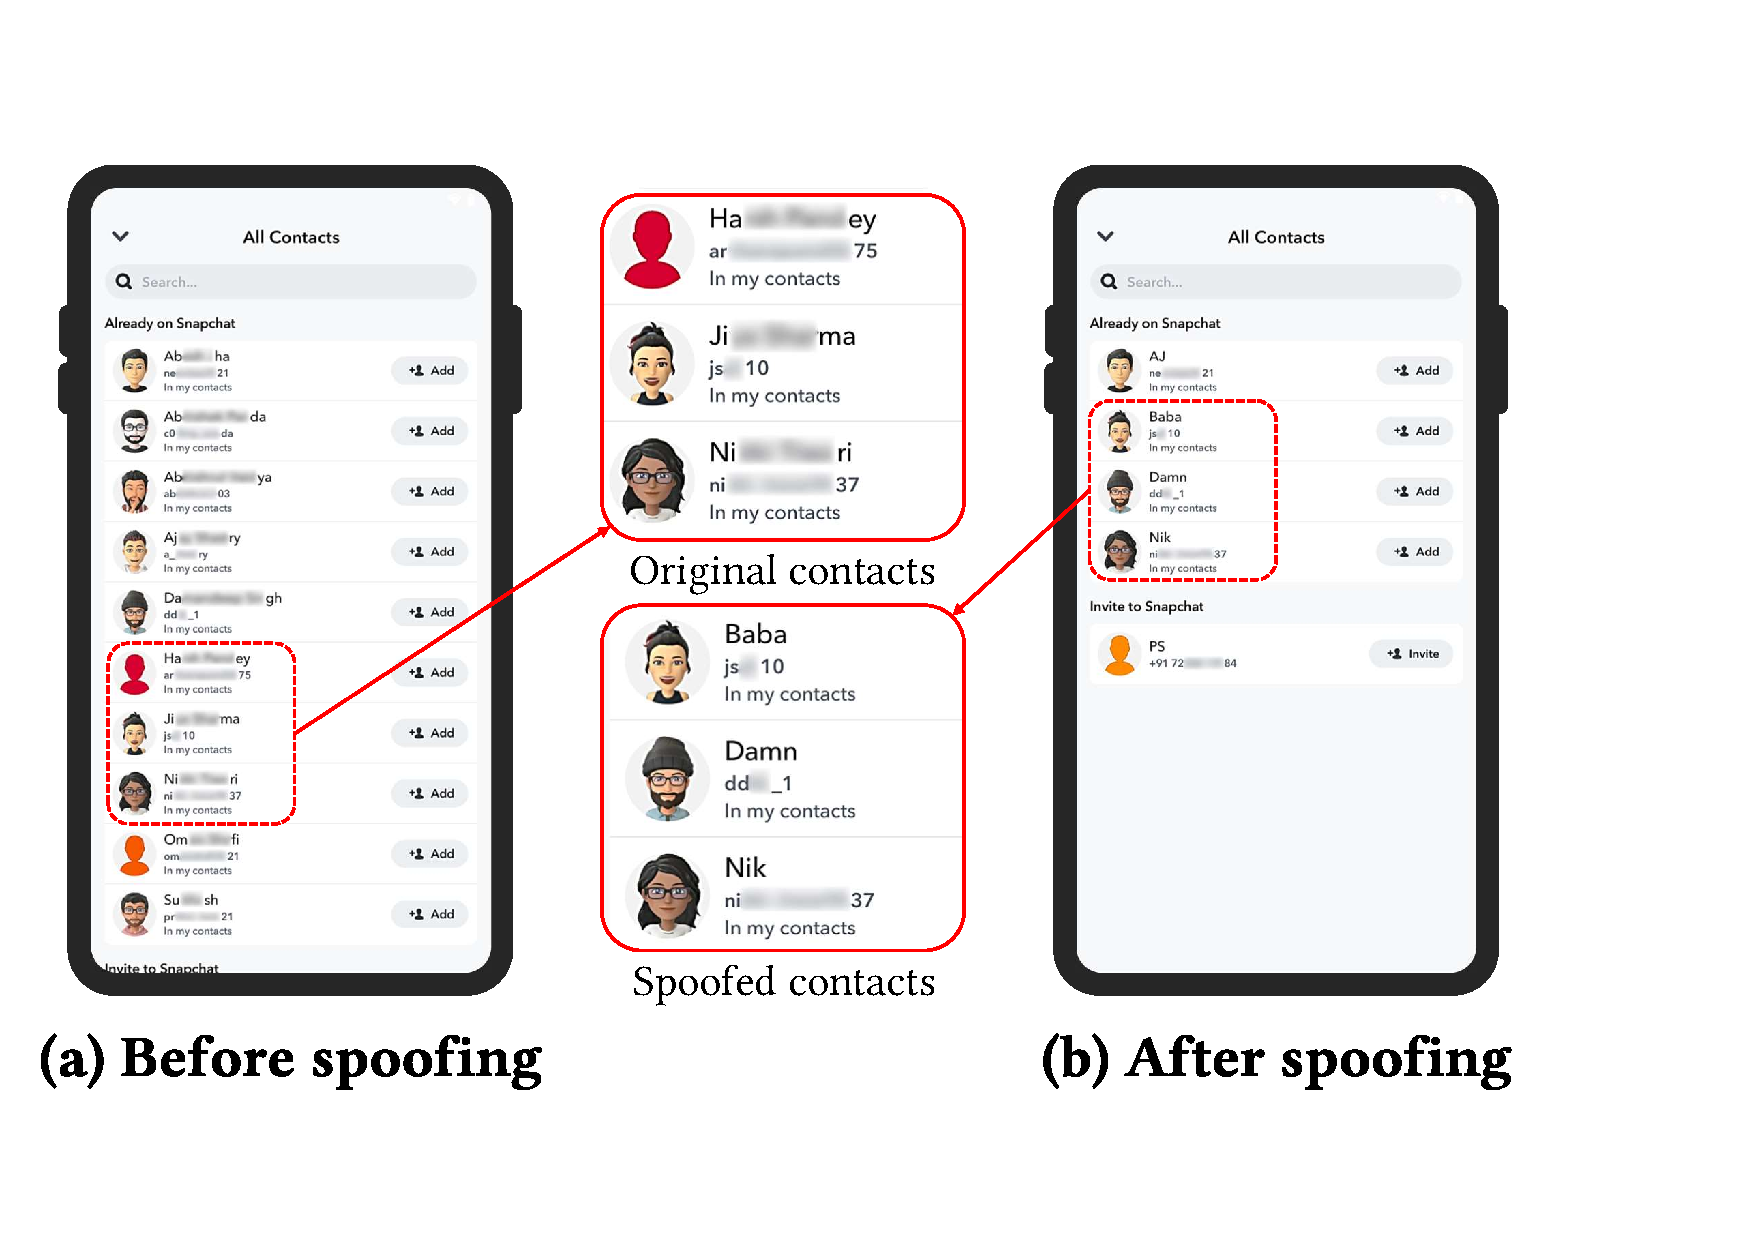
\includegraphics[width=0.75\linewidth]{Figures/Case Studies/snapchat_screenshots.pdf}
    \caption{Screenshots demonstrating how user can share spoofed contacts using WhiteLie with Snapchat.}
    \label{fig:case-study-snapchat}
\end{figure}

Snapchat has a feature called \textit{Snap Map}, which utilizes the device's GPS and other sensors to display user avatars on a map, showcasing real-time physical activities. While Snapchat does provide \textit{Ghost Mode} as an option to refrain from sharing location and sensor data, it sacrifices \textit{SnapMap} features that rely on this information. Furthermore, \textit{Ghost Mode} does not guarantee that the app is not accessing the data. 

\framework{} successfully spoofed device's GPS location and \texttt{READ\_CONTACTS} by utilizing a list of contacts specified in \framework{}'s \textit{Deceit} section as shown in Figure \ref{fig:case-study-snapchat}(b). Users can thus limit the information they want to share with Snapchat and still use Snap Map feature.

\subsection{com.truecaller (v12.54.7)}
\label{sec:tc_case_study}
Truecaller provides sender information about incoming text messages to highlight known spammers. With Truecaller, users can ignore spam messages. But to use this feature, users have to give permission to the app to read all their messages. We used \framework{} to successfully spoof message content while retaining the phone number from which the message was received. This way users can retain control over the privacy of their messages while still identifying whether senders are known spammers as shown in
Figure~\ref{fig:case-study-truecaller}(b).

\begin{figure}[t]\centering
    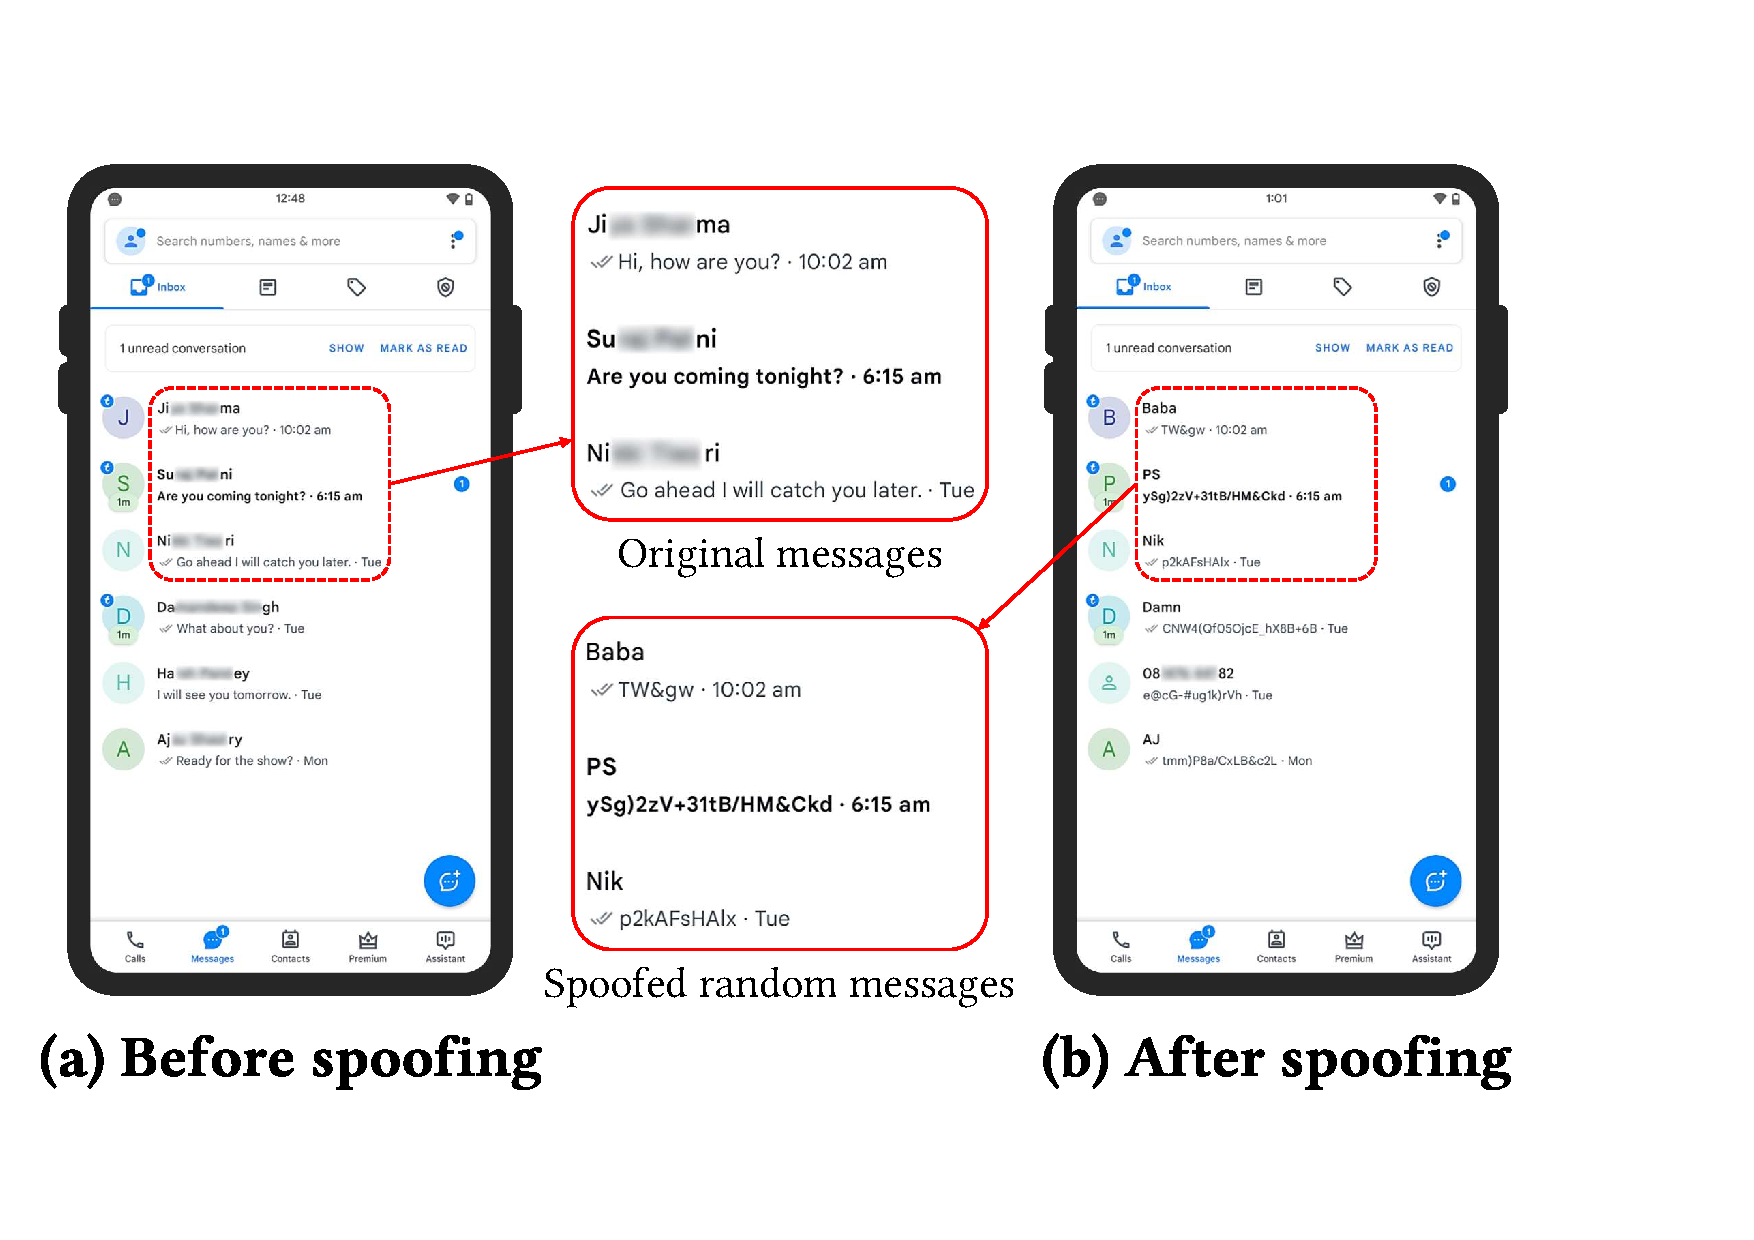
\includegraphics[width=0.75\linewidth]{Figures/Case Studies/truecaller_screenshots.pdf}
    \caption{Screenshots demonstrating how a user can share spoofed SMS using WhiteLie with Truecaller app.}
    \label{fig:case-study-truecaller}
\end{figure}

\textit{Overall, this section shows that \framework{} empowers users to fully use the app features while controlling the information that they share with the apps.}

\newpage
\section{Defending against Malware Attacks}
\label{sec:mitigating_sca}

% For instance, Hasan~\cite{hasan2013sensing} demonstrated a side-channel attack that enables a target device to communicate covertly with nearby devices using the magnetic sensor without the user's knowledge or consent. PIN Skimmer~\cite{simon2013pin} exploits camera and microphone recordings of a smartphone's virtual keypad to predict entered PINs with 50\% accuracy. AccelEve~\cite{ba2020learning}, utilizing the broad range of human speech captured by accelerometers, employs advanced side-channel attacks to eavesdrop on the device's onboard speaker and reconstruct audio recordings using deep learning techniques. Additionally, Shen~\cite{shen2015input} presented a machine-learning model that accurately predicts user touch and swipe gestures by analyzing accelerometer and magnetometer sensor data.

% To uphold robust security measures on Android devices, it is imperative to
% understand and mitigate emerging attacks that compromise user privacy.
In this section, we show that \framework offers a novel approach to mitigate the
risk of leaking sensitive user data.

\subsection{Testing \framework{} against Real-world Malicious Apps}
\label{sec:malicious_apps}

To analyze the defense capabilities of \framework
against real-world malicious apps, we selected 30 most downloaded apps 
that had been recently banned from Google Play
Store. Due to the absence of accessible downloads for banned apps on the Google Play
Store, we downloaded the latest versions available on third-party platforms. 
% We treated these apps as potentially infected with malware, similar to their Play Store counterparts. To conduct our analysis, we utilized a rooted device exclusively equipped with built-in apps, ensuring the complete removal of any injected malicious code after experiments.
% For these experiments, 
% we focused on a subset of permissions 
% %that the \framework{} could effectively deceive, 
% prioritizing protecting critical user data against such malicious apps. 
% To safeguard user privacy and data, we configured \framework{} to deceive these
% apps upon installation, ensuring no accurate information was shared. 
We then scrutinized the malicious behavior of these apps using the sensitive API
access logs captured by the \framework.

\begin{table}
    {\centering
    % \begin{tabular}{>{\arraybackslash} m{4.1cm}  >{\centering\arraybackslash} m{2cm} >{\centering\arraybackslash} m{5.15cm} >{\centering\arraybackslash} m{5.15cm}}
    \begin{tabular}{p{\linewidth}} 
         \toprule
         \textbf{Malicious behavior:} Upload sensitive data to internet\\
         \textbf{Apps (downloads):}
         All Good PDF Scanner (10M+), Fast PDF Scanner (5M+), PhoneFinder by
         Clapping (5M+), What's Me Sticker (1M+)\\
         \textbf{\framework:} Limit internet access to the app\\
         \midrule
         \midrule
         \textbf{Malicious behavior:} Access sensitive user data like Contacts, Location, Audio,
         and Sensors unnecessarily\\
         \textbf{Apps (downloads):} Amazing Video Editor (5M+), CapCut Pro (5M+), Instant Speech Translation (5M+), Keyboard Themes (5M+),
         Launcher iOS 15 (5M+) \\
         \textbf{\framework:} Deceived all the unnecessary user data requested without crashing the apps\\
         \midrule
         \midrule
         \textbf{Malicious behavior:} Accessing data without user knowledge\\
         \textit{Accessing sensor data in the background}\\
         \textbf{Apps (downloads):} Bus Driver Simulator (5M+), Bus - Metrolis 2021 (1M+),
         Fingerprint Changer (1M+), Fingerprint Defender (1M+), Lifeel - scan and test (5M+),
         Locker Tool (5M+), OFFRoaders - Survive (5M+), Racers Car Driver (5M+), Safe Lock (5M+),
         Slime Simulator (5M+), Smart Spot Locator (1M+), Unique Keyboard (5M+) \\
         \textbf{\framework:} Allowed the apps to access the sensor
         data in the foreground but not in the background\\
         \midrule
         
         \textit{Camera access without user consent and knowledge}\\
         \textbf{Apps (downloads):} Free Translator Photo (5M+), Handy Translator Pro (10M+),
         Heart Rate and Pulse Tracker (5M+), Heart Rhythm (1M+),
         My Chat Translator (5M+) \\
         \textbf{\framework:} Deceived camera data fed into the app\\
         \midrule
         
         \textit{Location continuously tracked by app}\\
         \textbf{Apps (downloads):} Geospot: GPS Tracker (5M+), iCare - Find Location (5M+) \\
         \textbf{\framework:} Deceived location data according to user policy\\
         \midrule
        \midrule
        \textbf{Malicious behavior:} Detected accessing Send SMS API without user knowledge\\
        \textbf{Apps (downloads):} Private SMS (5M+), Mint Left Messages (1M+) \\
        \textbf{\framework:} Blocked access to send SMS but not from reading SMS as per user policy\\
        \bottomrule
    \end{tabular}
    }
    \caption{Malicious behavior of Android apps banned by Google and the actions taken by \framework 
    to protect user privacy.}
    \label{tab:malicious_apps}
\end{table}

% \begin{table*}
%     {\centering
%     \begin{tabular}{>{\centering\arraybackslash} m{4.1cm}  >{\centering\arraybackslash} m{2cm} >{\centering\arraybackslash} m{5.15cm} >{\centering\arraybackslash} m{5.15cm}}
%         \hline
%          \textbf{Malicious App} & \textbf{\#Downloads (in millions)} & \textbf{Malicious activities detected by \framework{}} & \textbf{Actions performed by \framework{}} \\
%          \hline
         
%          All Good PDF Scanner & 10+ & Cam, Net & SUP(Cam), SB\\
%          Fast PDF Scanner & 5+ & Cam, Net & SUP(Cam), SB \\
%          PhoneFinder by Clapping & 5+ & Net, Aud & SUP(Aud), UDP(Net), SB \\
%          What's Me Sticker & 1+ & Cam, Net & SUP(Cam), UDP(Net), SB \\
%          \hline         
         
%          Amazing Video Editor & 5+ & Acc, Aud, Cam, Con, Loc, Net & SUP(Aud, Cam), UDP(Acc, Con, Loc), SB\\
%          CapCut Pro & 5+ & Aud, Cam, Con, Loc, Net & SUP(Aud, Cam), UDP(Con, Loc), SB\\
%          \hline
         
%          Bus Driver Simulator & 5+ & Net & UDP(Net), SB \\
%          Bus - Metrolis 2021 & 1+ & Net & UDP(Net), SB \\
%          Fingerprint Changer & 1+ & Net & SB \\
%          Fingerprint Defender & 1+ & Net & SB \\
%          Lifeel - scan and test & 5+ & Net & SB \\
%          Locker Tool & 5+ & Net & UDP(Net), SB \\
%          OFFRoaders - Survive & 5+ & Net & UDP(Net), SB \\
%          Racers Car Driver & 5+ & Net & UDP(Net), SB \\
%          Safe Lock & 5+ & Net & UDP(Net), SB \\
%          Slime Simulator & 5+ & Net & UDP(Net), SB \\
%          Smart Spot Locator & 1+ & Net & SB\\
%          Unique Keyboard & 5+ & Net & UDP(Net), SB \\
%          \hline

%          Private SMS & 5+ & Acc, Cam, CLg, Con, Msg, Net & SUP(Acc, Cam, CLg, Con, Msg), SB\\
%          Mint Left Messages & 1+ & Aud, Cam, CLg, Con, Msg, Net & SUP(Aud, CLg, Cam, Con, Msg), SB\\
%          \hline
         
%          Free Translator Photo & 5+ & Cam & SUP(Cam), SB \\
%          Handy Translator Pro & 10+ & Acc, Cam & UDP(Acc), SUP(Cam), SB \\
%          My Chat Translator & 5+ & Acc, Cam & UDP(Acc), UDU(Cam), SB \\
%          \hline
         
%          Geospot: GPS Tracker & 5+ &  Loc, Net  & SUP(Loc), SB \\
%          iCare - Find Location & 5+ &  Cam, Loc, Net  & SUP(Loc), UDP(Cam), SB\\
%          \hline
         
%          Heart Rate and Pulse Tracker & 5+ & Cam & UDP(Cam), SB \\         
%          Heart Rhythm & 1+ & Cam & UDP(Cam), SB \\
%          \hline
         
%          Instant Speech Translation & 5+ & Acc, Aud, Cam & UDP(Acc, Cam), SUP(Aud), SB \\
%          \hline
         
%          Keyboard Themes & 5+ & Acc, Con & UDP(Acc, Con), SB \\
%          Launcher iOS 15 & 5+ & Acc, Aud, Cam, Con, Loc, Net & UDU(Acc, Aud, Cam, Con, Loc, Net), SB \\
%          \hline
         
         
         
         
         
         

%          \hline
%          \multicolumn{4}{l}{\footnotesize \textbf{Acc}: Account, \textbf{Aud}: Audio, \textbf{Cam}: Camera, \textbf{CLg}: Call Logs, \textbf{Con}: Contacts, \textbf{Loc}: Location, \textbf{Msg}: SMS, \textbf{Net}: Network } \\
         
%          \hline
%          \multicolumn{4}{p{16.4cm}}{\footnotesize \textbf{SB}: Sandboxing apps and isolating from external world and other apps installed on the device to protect user privacy and mitigate attacks, \textbf{SUP}: Selective user data protection to ensure app functionality without compromising user data, \textbf{UDP}: Deceiving unnecessary dangerous permissions requested to ensure user privacy without crashing app, \textbf{UDU}: Detecting and blocking unexpected user data usage } \\
%          \hline
%     \end{tabular}
%     }
%     \caption{Malicious Android Apps banned by Google.}
%     \label{tab:malicious_apps}
% \end{table*}

Table \ref{tab:malicious_apps} summaries the list of malicious behaviors we found 
in the 30 malicious apps. We expect users to be able to find malicious behaviors
in a similar manner. In future, we plan to extend \framework to notify users upon 
suspected malicious behaviors.
% malicious apps banned by
% Google and tested using \framework{} along with the malicious behavior detected
% and the corresponding action. 

Malicious behaviors fell under 6 categories:

\noindent\textbf{\textit{Upload sensitive data to the internet.}} Some apps were
identified for transmitting substantial amounts of data over the internet while
operating in the background. For example, we suspect \textit{PhoneFinder by
Clapping} was uploading user audio data as it had also been granted audio
permission. We could not revoke or spoof audio permission without hurting the
app's functionality. Consequently, \framework limited the app's internet access
to safeguard user privacy.

\noindent\textbf{\textit{Accessing sensitive data unnecessarily.}} A typical
pattern among malicious apps was to try to access irrelevant sensitive data. For
example, \textit{Amazing Video Editor} and \textit{Keyboard Themes} apps were
accessing user's contacts information. Similarly, \textit{Instant Speech
Translation} was accessing user's photos. Denying requests for these permissions
led to crashes or termination of the apps. \framework could successfully spoof
such unnecessary sensitive data accessed by these apps without limiting app
functionality.

\noindent\textbf{\textit{Accessing data without user knowledge.}} Other apps 
were calling sensitive APIs at unexpected times. For example, \textit{Free
Translator Photo} app translates images uploaded by the user. However, the app
was found to attempt access to user images even when user had not requested a
translation. \textit{Bus Driver Simulator} allows users to play a game using
accelerometer and gyroscope sensor data. But the app was accessing the sensors
while it was in background. \framework could effectively deceive all the
sensitive data including camera, audio, contacts, location, sensors, and device
information. Users can easily configure deceiving policies to deceive only while
the app is in background while allowing sensitive data while the app is in
foreground.

\textit{GeoSpot: GPS tracker} can let users share their current location with
friends. However, it was found to track the user even when the user has not
asked the app to share their location. \framework could effectively deceive the
location of the user. But since both regular and malicious operations happen
while app is in background, user has to enable/disable deceiving manually with
\framework.

% Additionally, some apps that
% continued to function despite being denied permission requests, repeatedly
% prompted for permissions during the interaction. Reviews on third-party app
% stores echoed similar experiences, raising suspicions about these apps. Another
% noteworthy observation was the peculiar nature of the requested permissions. For
% instance, apps belonging to a specific domain requested permissions irrelevant
% to their intended functionality, such as a theme app requesting access to
% contacts information.

% To examine the mechanisms and signatures employed by these apps for malicious
% activities, we granted and extensively used all requested permissions. The apps
% appeared to function normally after obtaining the permissions, and no immediate
% cause for concern was apparent during user interaction. However, inspecting the
% logs, we discovered that these apps accessed unnecessary user data, such as
% , in the background while performing intended tasks. Fortunately, \framework{}
% effectively logged
% and deceived these data requests with the values defined in the \textit{Policy
% Configurator}. 

\noindent\textbf{\textit{Sending SMS messages.}} Some apps like \textit{Private
SMS} call \texttt{SMSManager.sendTextMessage()} without user consent.
Multiple media reports suggest that such apps commit financial fraud by
subscribing users to premium services through SMS activation. \framework
prevented sending these messages from the device. However, doing so also limits
the app's functionality. \framework is therefore not effective where the app
does malicious activities using the data needed for its core functionalities. 


\subsection{Mitigating Side-Channel Attacks}
\label{sec:side_channel_attack}
Side-channel attacks present a significant threat to the security of mobile devices. These attacks exploit unintentional channels of information leakage, such as accelerometers, gyroscopes, power consumption, or electromagnetic radiation, to infer sensitive data. With their abundance of sensors and communication interfaces, mobile devices are particularly vulnerable to side-channel attacks. These attacks can lead to the unauthorized disclosure of valuable information like passwords, cryptographic keys, or biometric data.

Recent studies~\cite{hasan2013sensing, simon2013pin, ba2020learning, shen2015input} have shed light on the risks associated with so-called \textit{Normal} Permissions, which include seemingly innocuous actions like reading sensor data that do not require explicit user approval. However, in various attacks on user privacy, these permissions are leveraged. 

In response to the pressing privacy concern, our framework offers a novel approach to mitigate the risk of side-channel attacks perpetrated by malicious apps. By selectively modifying permissions granted to specific apps, \framework{} fortifies user privacy and bolsters mobile device security. \framework{} achieves this by deceiving user data, effectively disrupting the ability of malicious apps to gather sensitive information through side-channel channels.

We showcase the effectiveness of the \framework{} in countering the insidious side-channel attacks, by conducting tests employing \textit{GyroSec}~\cite{lin2019motion}. \textit{GyroSec} is an Android application that captures readings from the device's accelerometer and gyroscope without the user's knowledge or consent. This unauthorized data is then transmitted to a remote server where \textit{GyroSec} employs machine-learning algorithms to discern and predict the precise location of touch inputs on the screen. This capability poses a significant danger, as it leads to leakage of users' sensitive information. Our experiments have uncovered that \textit{GyroSec} can carry out such side-channel attacks without any restrictions from the Android Permission Framework.

% \begin{figure}[t]
% \centering
% \begin{subfigure}{0.4\linewidth}
%     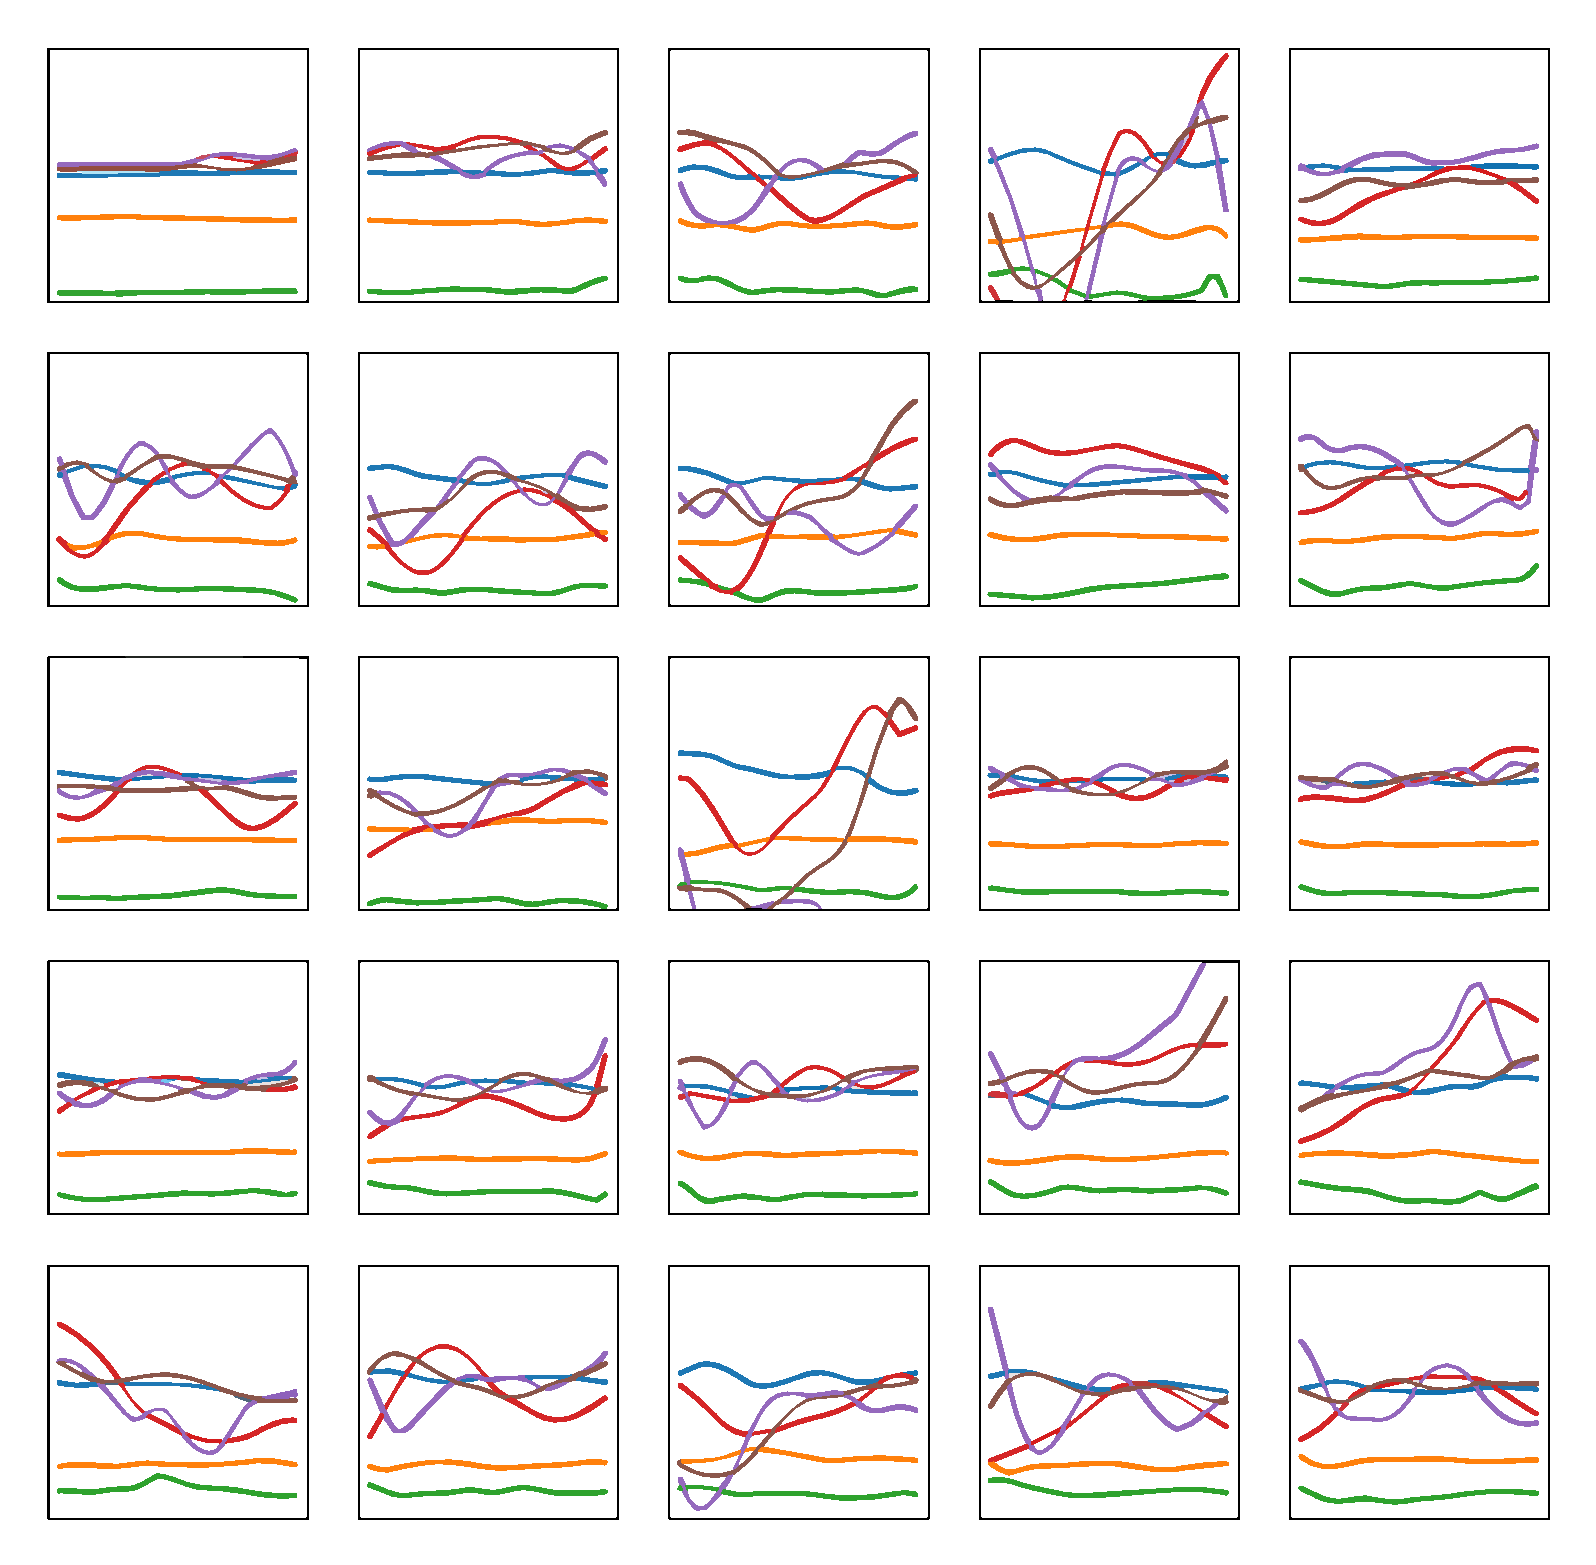
\includegraphics[width=\linewidth]{figures/side_channel_attack_results/sensor_data_non_touch_samples_received_at_GyroSec_server_without_Deceiver.pdf}
%     \caption{Non-touch samples without \framework{}}
%     \label{fig:dataSampleGyroSec_ntwoF}
% \end{subfigure}
% \hspace{0.9mm}
% \begin{subfigure}{0.4\linewidth}
%     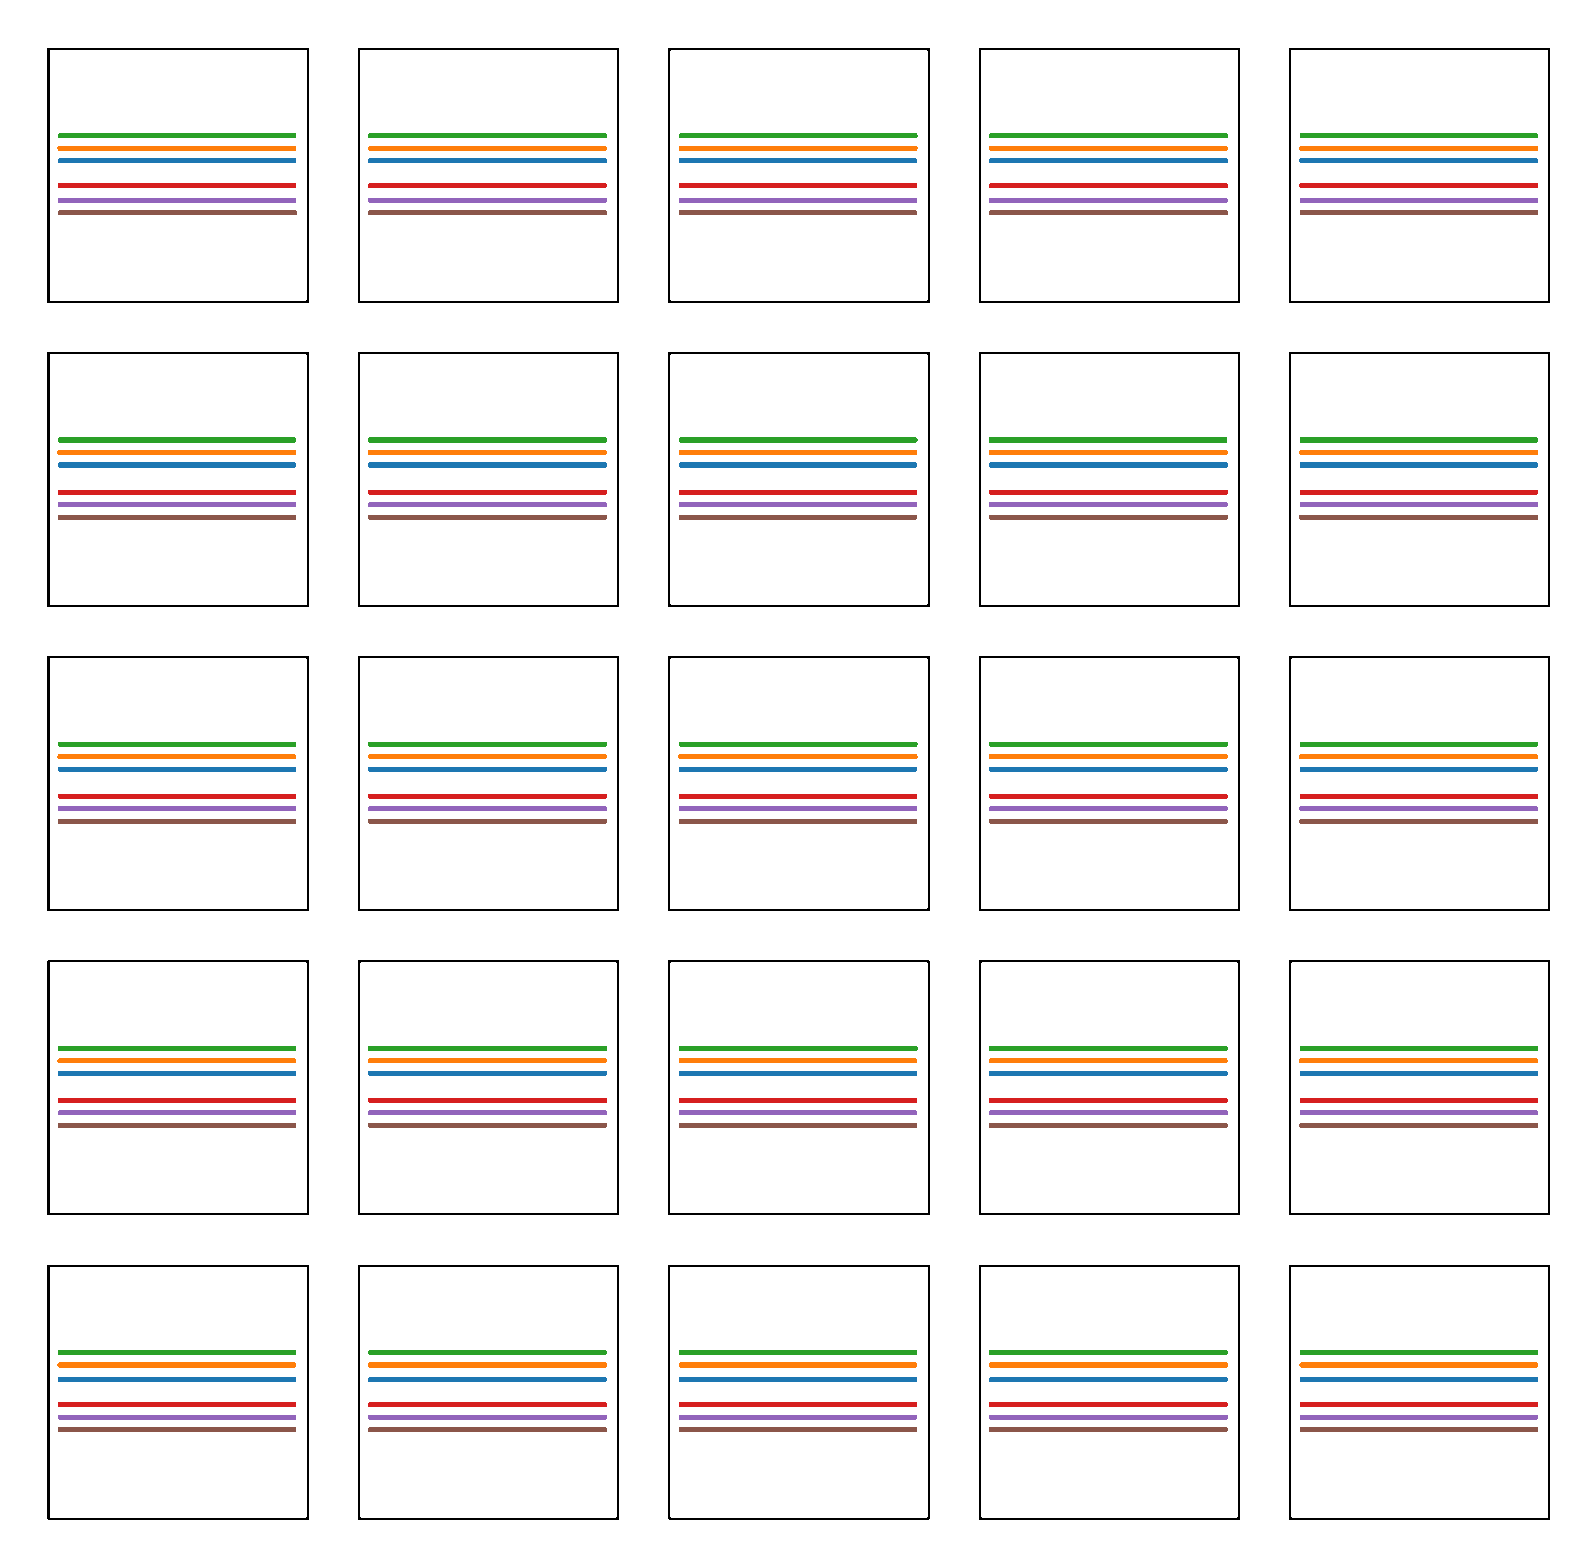
\includegraphics[width=\linewidth]{figures/side_channel_attack_results/sensor_data_non_touch_samples_received_at_GyroSec_server_with_Deceiver.pdf}
%     \caption{Non-touch samples with \framework{}}
%     \label{fig:dataSampleGyroSec_ntwF}
% \end{subfigure}
% \begin{subfigure}{0.4\linewidth}
%     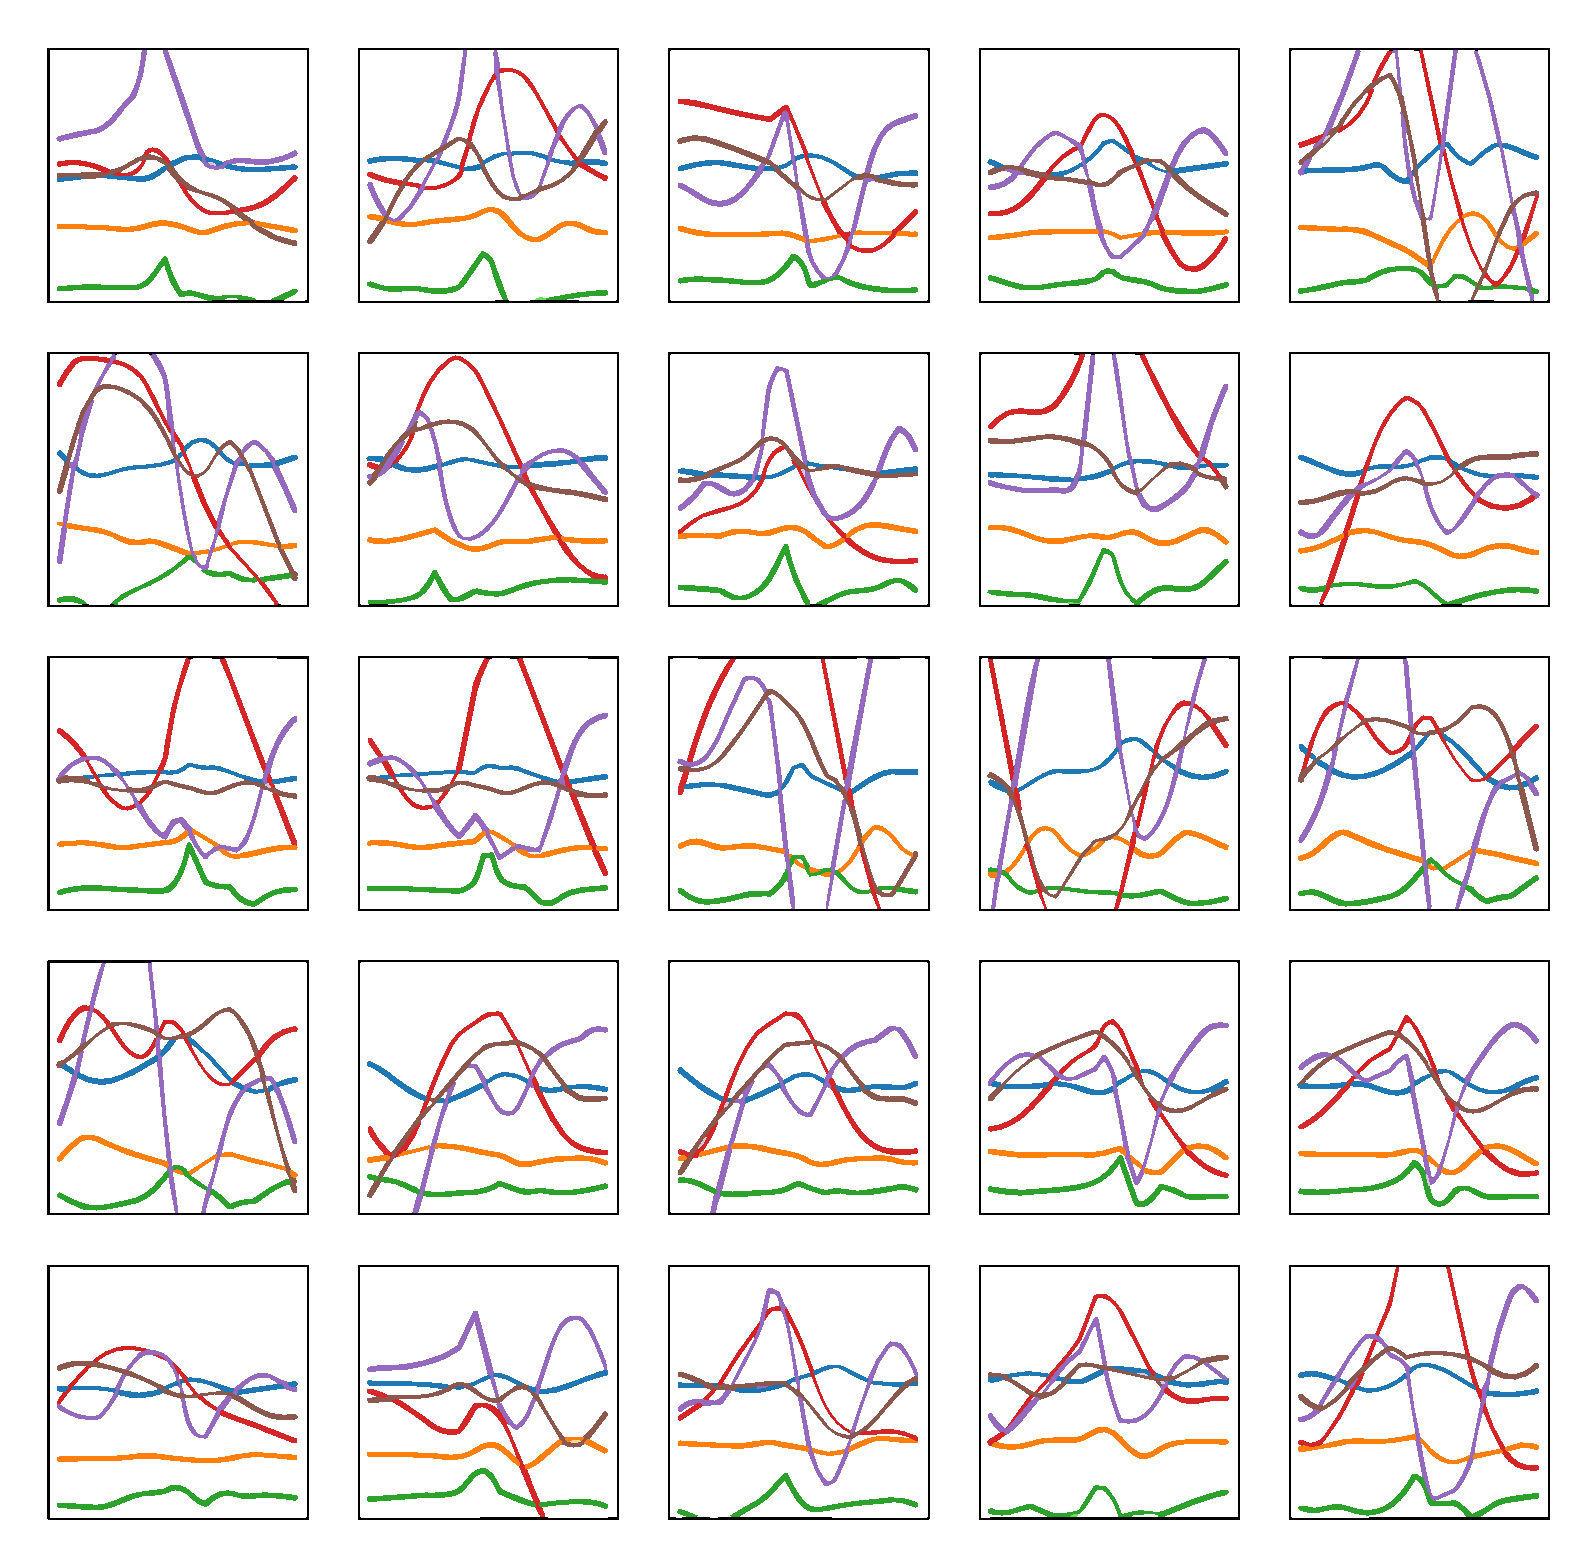
\includegraphics[width=\linewidth]{figures/side_channel_attack_results/sensor_data_touch_samples_received_at_GyroSec_server_without_Deceiver.pdf}
%     \caption{Touch samples without \framework{}}
%     \label{fig:dataSampleGyroSec_twoF}
% \end{subfigure}
% \hspace{0.9mm}
% \begin{subfigure}{0.4\linewidth}
%     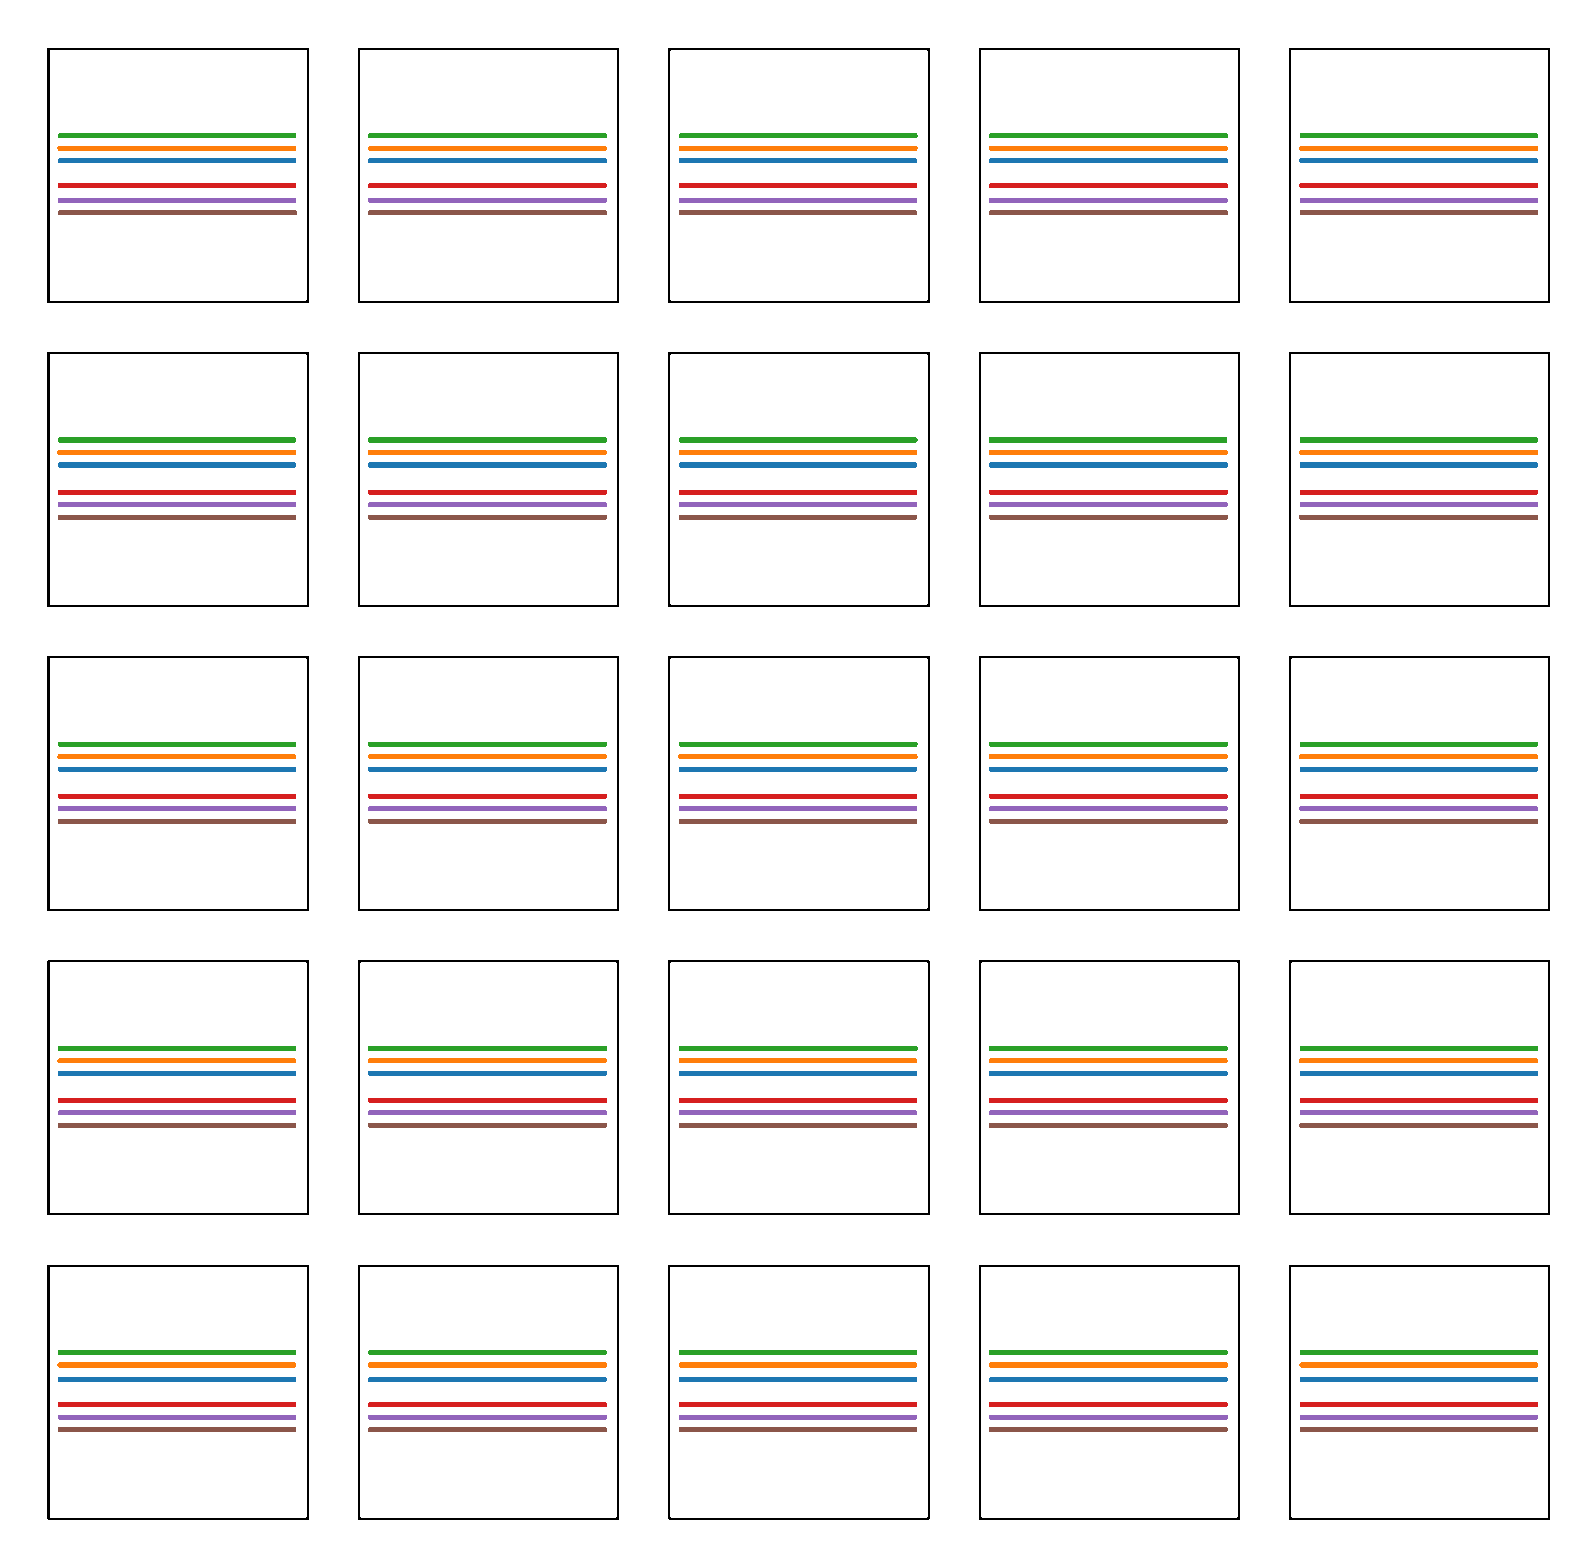
\includegraphics[width=\linewidth]{figures/side_channel_attack_results/sensor_data_touch_samples_received_at_GyroSec_server_with_Deceiver.pdf}
%     \caption{Touch samples with \framework{}}
%     \label{fig:dataSampleGyroSec_twF}
% \end{subfigure}
% \caption{Samples of Accelerometer and Gyroscope sensor data readings received at server.}
% \label{fig:dataSampleGyroSec}
% \end{figure}

%Nevertheless, our resolute experiments have demonstrated the defense mechanisms of the \framework{} against these side-channel attacks. 
By configuring \framework{} to deceive \textit{GyroSec}, we logged every instance of data access by \textit{GyroSec}, promptly notifying users of any background resource data breaches. \framework{} further deceived the data received by \textit{GyroSec}. Using the \textit{Policy Configurator} the accelerometer and gyroscope sensor readings were deceived as constant value for Gyrosec.
% It cleverly made the data harder to understand by using carefully chosen values set up in the \framework{}'s \textit{Policy Configurator}. As a result, \textit{GyroSec}'s server was rendered utterly impotent in its feeble attempts to predict touch positions, endowing users with unwavering privacy protection. 
Figure \ref{fig:tchPredict} illustrates reduction in \textit{GyroSec}'s ability to predict accurately by \framework{}. The prediction accuracy dropped from \textbf{81.22\%} to \textbf{5.36\%}, proving \framework{} to be a successful measure against Permission-based Side-Channel Attacks.

\begin{figure}[t]
\centering
\begin{subfigure}{0.35\linewidth}
    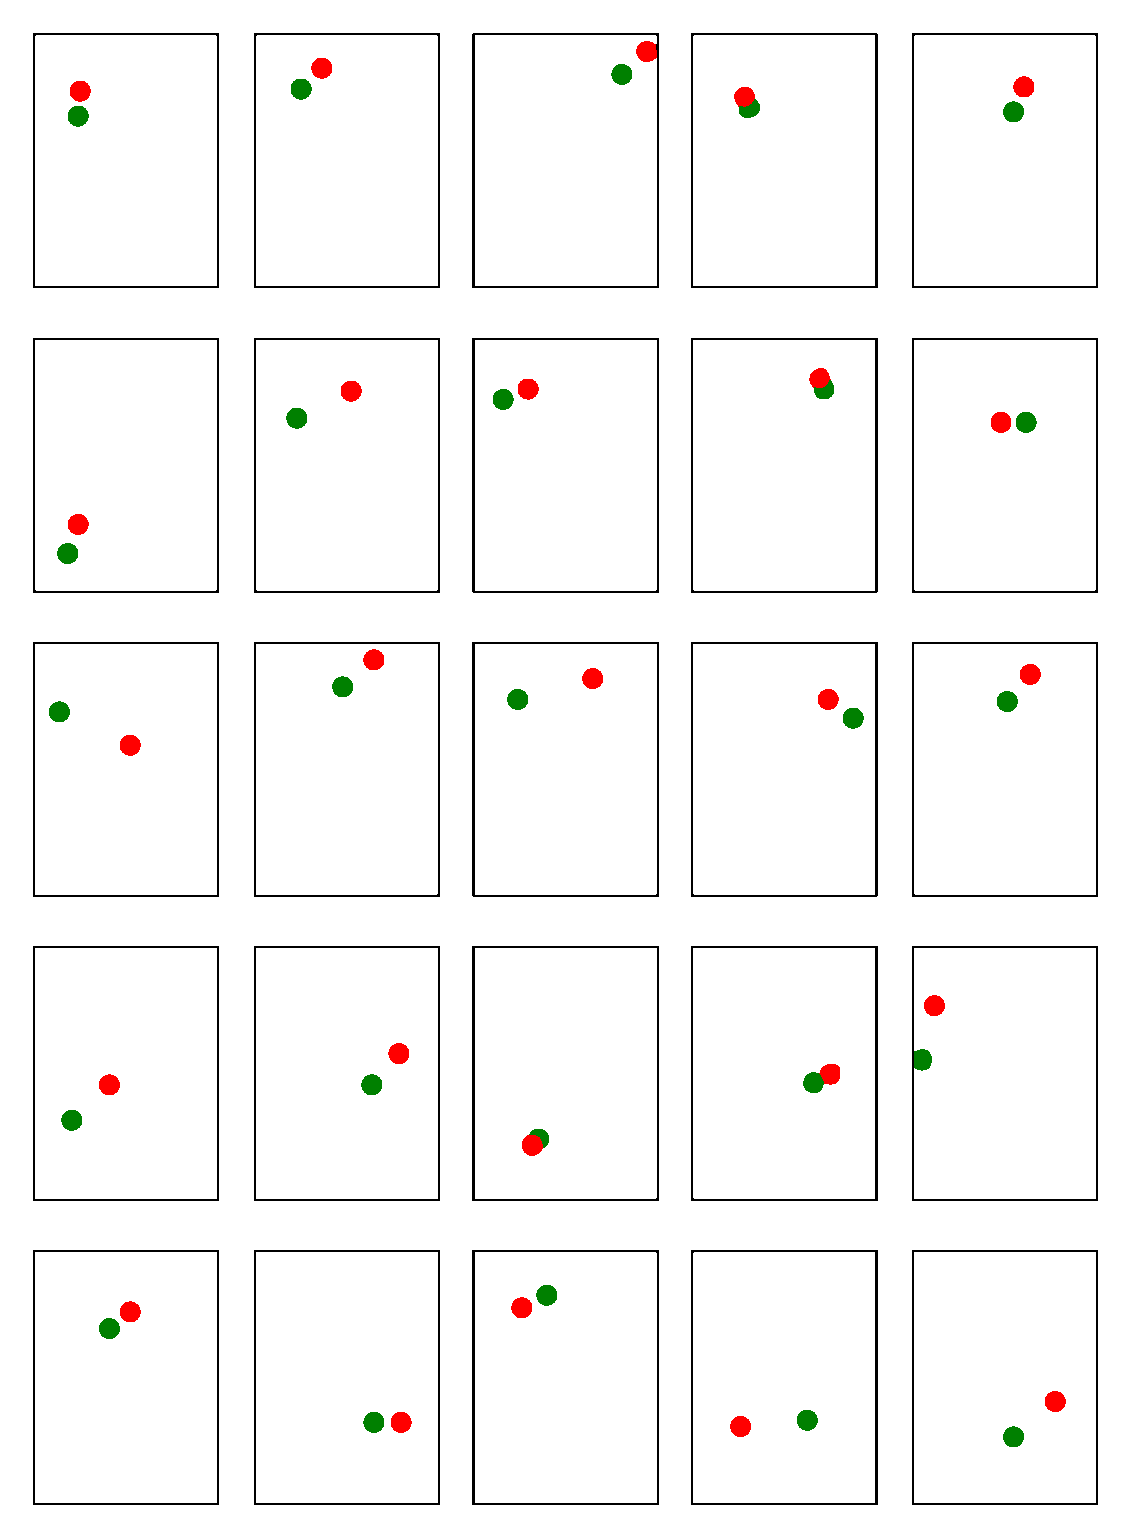
\includegraphics[width=\linewidth]{Figures/Side Channel Attacks/touch_prediction_samples_by_GyroSec_without_Deceiver.pdf}
    \caption{Without \framework{}}
    % \caption{Without \framework{} (High Accuracy achieved using true sensor readings)}
    \label{fig:tchPredict_wo_frmwrk}
\end{subfigure}
\hspace{0.9mm}
\begin{subfigure}{0.35\linewidth}
    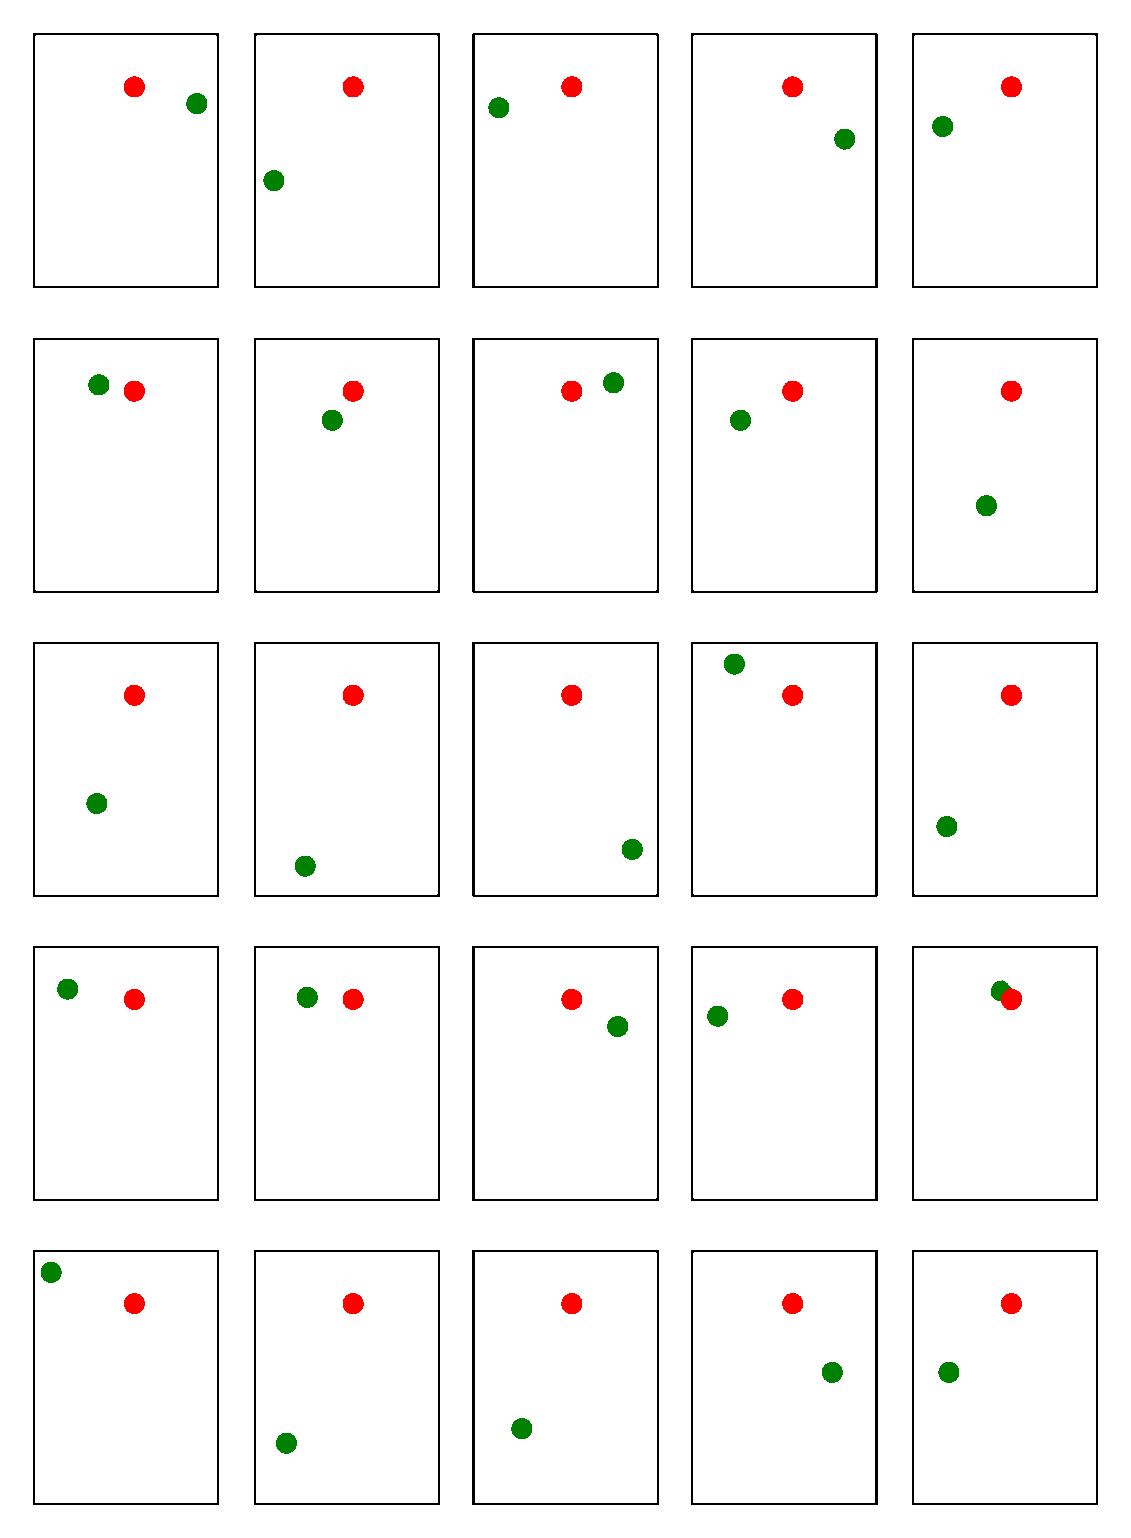
\includegraphics[width=\linewidth]{Figures/Side Channel Attacks/touch_prediction_samples_by_GyroSec_with_Deceiver.pdf}
    \caption{With \framework{}}
    \label{fig:tchPredict_w_frmwrk}
\end{subfigure}
\caption{Touch predicitions made by \textit{Gyrosec} server based on sensor readings received.}
\label{fig:tchPredict}
\end{figure}

%Hence, \framework{} counters Android side-channel attacks exploiting user data by manipulating the data the malicious app receives. The spoofed data compromises the integrity of the malicious server's results, rendering these attacks futile in gathering meaningful information about the user. 


\textit{Overall, this section shows that \framework could effectively stop most 
malicious behaviors giving better control to users over their sensitive data.}

% Based on the logs generated by \framework, we can confidently
% state that it effectively safeguards against malicious apps exploiting resource
% data for nefarious purposes.
\section{Evaluating Overhead}
\label{sec:results}

In this section, we present the outcomes of our evaluation of \framework{}, focusing on its performance overhead in a real device while running various real world apps.  We first quantify per API call overhead of \framework{} using micro-benchmarks. And then evaluate memory and battery overhead of \framework{} was evaluated using 10 most popular apps downloaded from the Google Play Store.

All permissions requested by the apps were granted beforehand, and the apps were subjected to 10 minutes of manual usage 5 times. All experiments were conducted on a \textit{Samsung Galaxy M21} smartphone with a 2.3 GHz octa-core processor and 4 GB of RAM running Android 12. 

\mysubsubsection{API call overhead}
We measure the time elapsed during code execution by executing hooked API methods within the \texttt{Timing.measureNanoTime()} method. We observed an average overhead of 1.64 ms across different API calls. The increase in elapsed time is because of the operations performed by the hooks. For user data like contacts and camera, we experienced an overhead of 3.87 ms and 3.23 ms respectively. For tracking and clipboard user data, we observed an overhead of 0.83 ms and 1.07 ms respectively. The overhead depends on the operations performed by the respective permission-deceiving hooks. For contacts and camera APIs, we are performing intensive operations like reading a database and manipulating pixels of an image, whereas for tracking and clipboard APIs, we are simply returning a deceived string. Many of these APIs were called several 

\begin{figure}[b!]
    \centering
    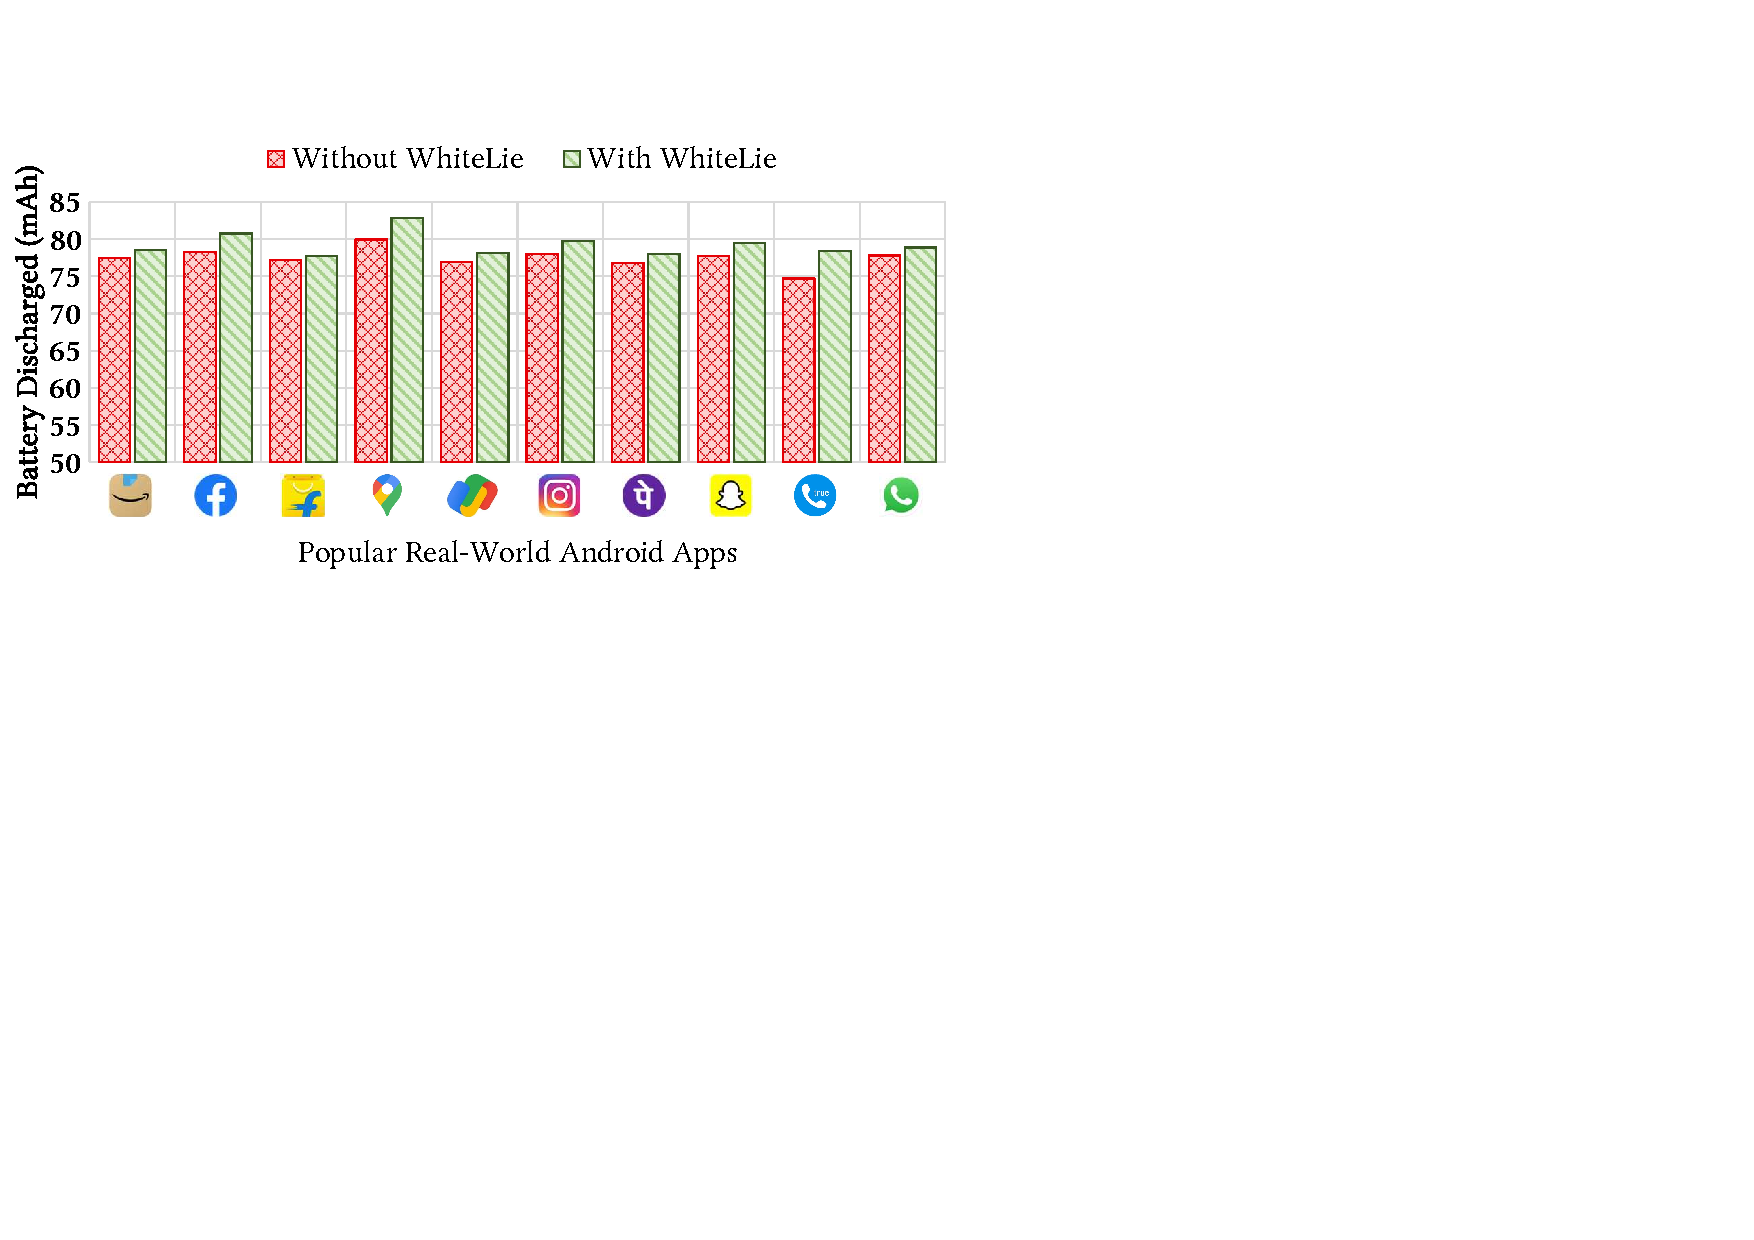
\includegraphics[width=0.8\linewidth]{Figures/Performance Evaluation/results_battery_discharged_real_world_apps.pdf}
    \caption{Battery discharged by various Android apps with and without \framework{}.}
    \label{fig:reslts_btryDschrgd}
\end{figure}

\noindent times during the app runs in our experiments. The API call overhead, however, did not impact the performance of the apps we tested in any observable manner. 

\mysubsubsection{Memory Used} 
The memory utilization of the benchmarking app was measured using \textit{ADB}'s \textit{dumpsys} tool, using the \textit{Proportional Set Size (PSS)} metric. This metric captures the shared memory proportionally used by each process. Figure~\ref{fig:results_memUsedAll} shows that on average, \framework{} only incurs 5.2 MB of memory overhead memory overhead while using \framework{} on various real-world apps.

\begin{figure}[t]
    % \vspace{-10pt}
    \centering
    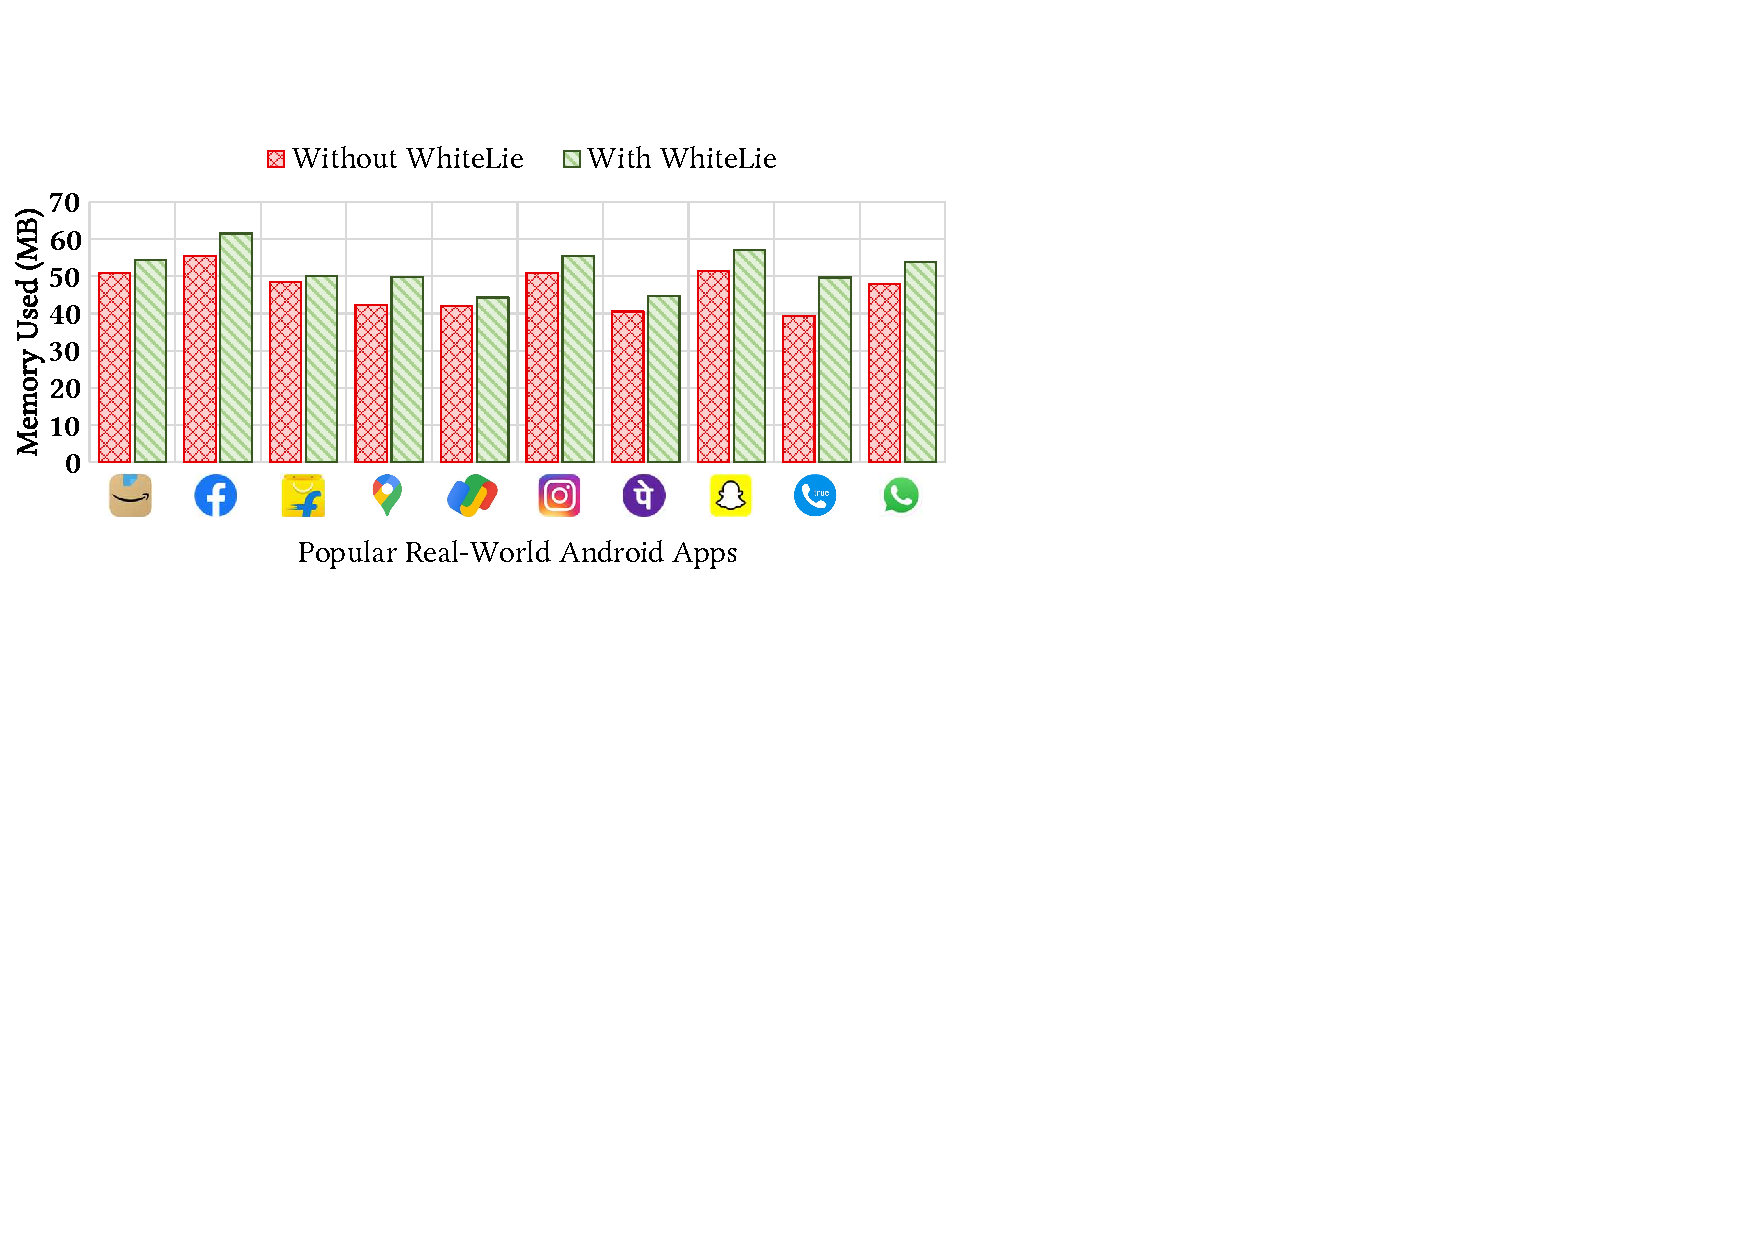
\includegraphics[width=0.8\linewidth]{Figures/Performance Evaluation/results_memory_used_target_app_real_world_apps.pdf}
    \caption{Memory used by various Android apps with and without \framework{}.}
    \label{fig:results_memUsedAll}
\end{figure}

\mysubsubsection{Battery Discharged}
To accurately measure the device's battery usage during our experiments, we utilized the \textit{ADB}'s \textit{batterystats} tool~\cite{batterystats}. 
% Before each experiment, we ensured a clean slate by resetting the tool. 
To mitigate any potential inconsistencies in battery usage statistics, we remotely connected the device via \textit{Wifi ADB}, as physically connecting it to a PC can inadvertently charge the device and yield inaccurate results.  By leveraging \texttt{batterystats}'s \textit{discharge} metric, we could quantify the amount of battery discharged since the last charge, accounting for the impact by both the target app and the system. Figure \ref{fig:reslts_btryDschrgd} shows that \framework{}'s impact on battery drain is negligible. An average additional discharge of approximately 1.76 mAh (2.52\%) was observed across 5 minutes runs of various apps, when they were run with \framework{}.

\begin{figure}[b!]
    \centering
    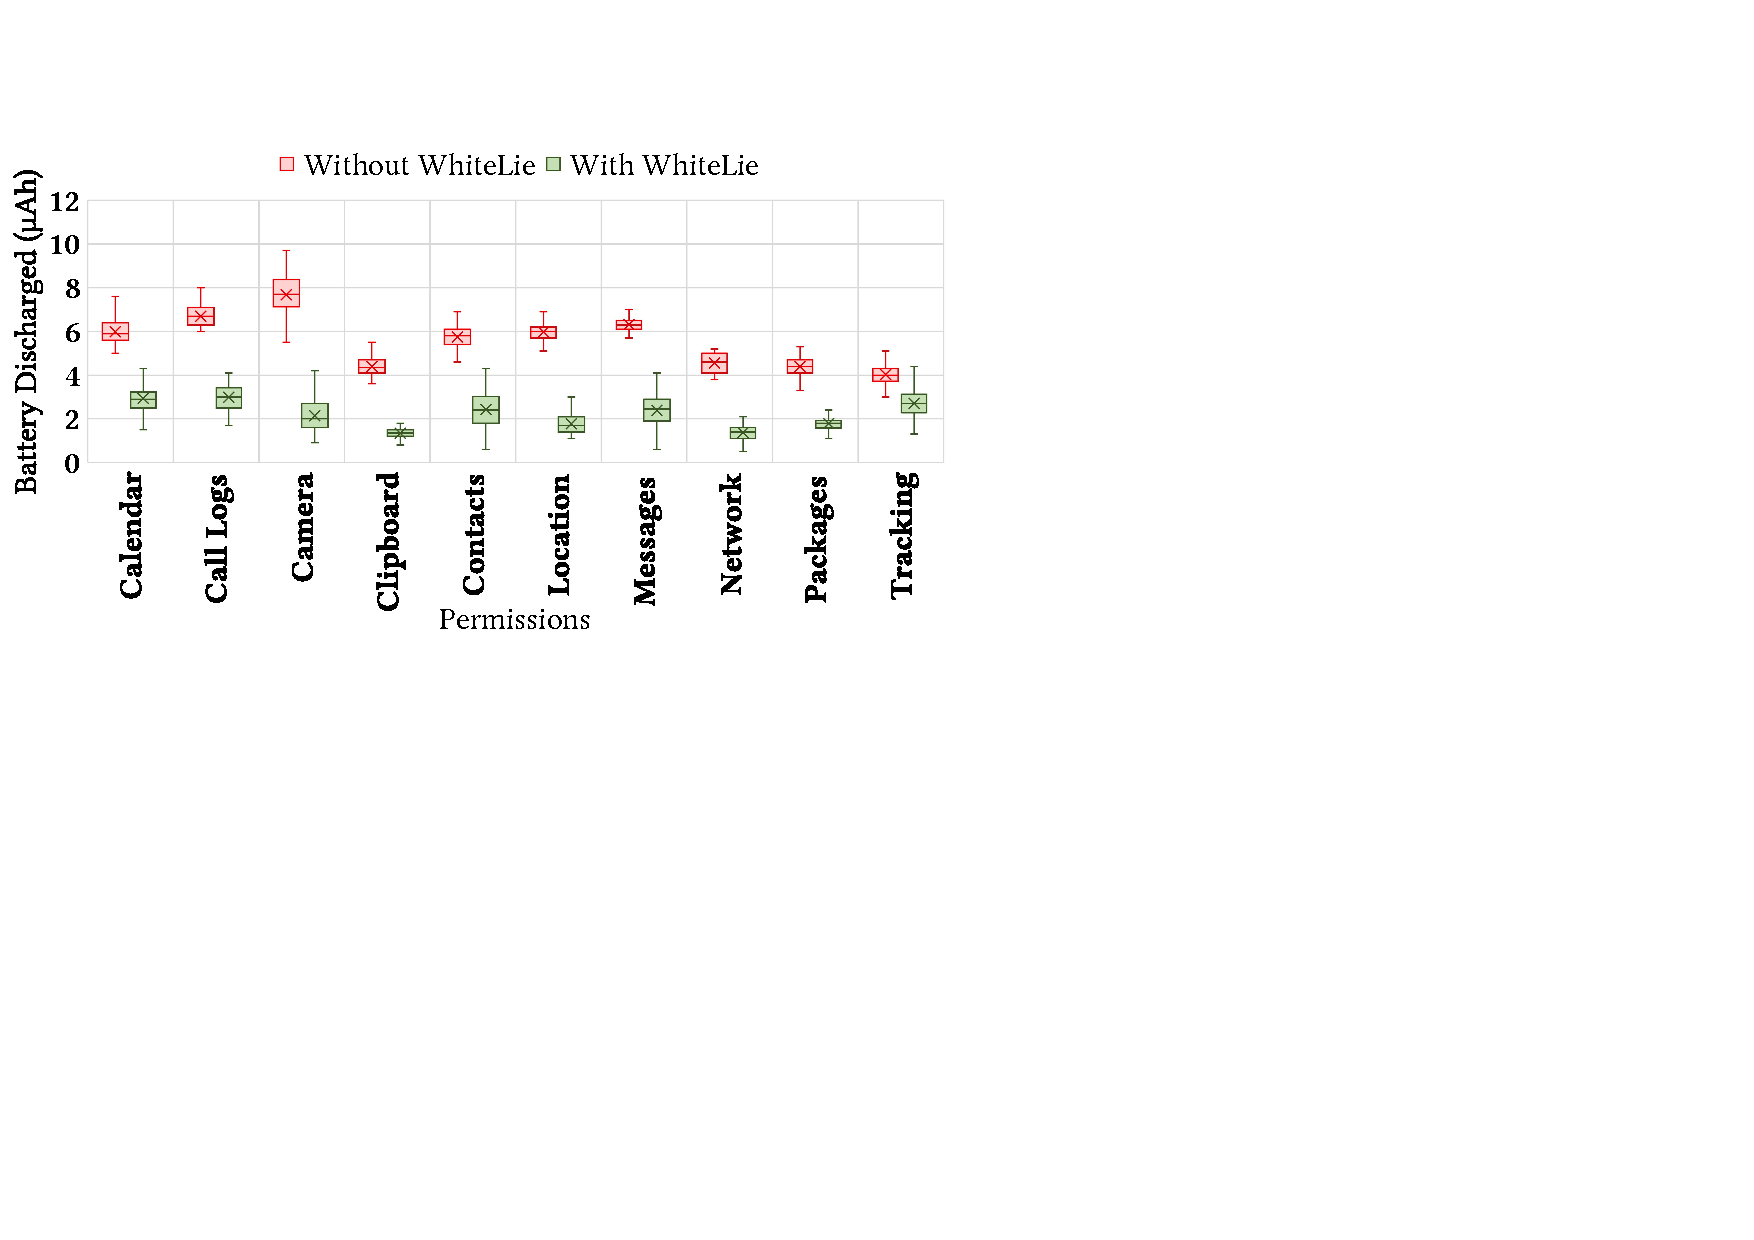
\includegraphics[width=0.8\linewidth]{Figures/Performance Evaluation/results_battery_discharged_battery_saver.pdf}
    \caption{Battery discharged by benchmarking app while fetching user data for various Permissions with and without \framework{} while using \textit{Battery Saver} mode.}
    \label{fig:reslts_btrySaver}
\end{figure}

  

\textit{Overall, our experiments show that \framework{}'s usage has a minimal impact on app's performance, memory consumption, and the device's battery drain. This shows that \framework{} is an efficient approach for protecting user privacy.}

We further experimented with actively reducing battery drain using \framework{}. In particular, by returning \texttt{null} from the \texttt{beforeHookedMethod()}, original method calls can be blocked which can save battery consumed by sensors and other components. To examine this, we added a battery saver mode to \framework{} that blocks Android API calls according to user policies. To measure the battery drainage, we developed a benchmarking app that performed a consecutive series of 1000 API calls to retrieve user data. We observed this approach saved an average of 4.08 $\mu{}Ah$ (60.83\%) per API call as illustrated in Figure~\ref{fig:reslts_btrySaver}.

\section{Related Work}
\label{sec:related_work}

Several past works~\cite{bokhorst2017xprivacy, bokhorst2021xprivacylua, hornyack2011these, ratazzi2019pinpoint, raval2019permissions, shrestha2016slogger} block or filter the user data to protect user's privacy. However, by spoofing the data instead of outright blocking or filtering it, provides users with greater control over their data without crashing the app.

Many approaches~\cite{backes2015boxify, jeon2012dr, raval2016you, smalley2013security, wu2017context} modify the Android OS or third-party app source code to deceive user data fed into apps. However, source code modification is detectable in modern Android OS making the tactic ineffective. In contrast, \framework{} eliminates the need for any modifications to the Android OS or third-party app source code.

Other approaches focus on improving the Android Permission Framework by offering intent of permission usage by the third-party apps ~\cite{chitkara2017does, tsai2017turtle, conti2011crepe, thanigaivelan2018codra}, momentarily revoking app permissions based on user-defined policies~\cite{bugiel2013flexible, liu2016follow, chakraborty2014ipshield}, app activities~\cite{zhang2015leave, chen2013contextual, chen2017sweetdroid, petracca2015audroid}, or machine learning algorithms~\cite{olejnik2017smarper, rashidi2016android, wijesekera2017feasibility, fu2017inspired}. Revoking permissions from Android apps comes at the cost of app crashes or limited app functionalities. Incorporating context-based policies, and machine learning algorithms to analyze app behaviour by generated logs with spoofing user data to ensure a seamless user experience and enhanced user privacy in \framework{} is an important future work.

% Current privacy protection methods based on context rely on revoking permissions and result in the loss of app functionalities, however incorporating context-based policies with spoofing user data instead of outright revocation would ensure a seamless user experience while maintaining a robust security mechanism.

% Relying solely on user-defined policies and log-based manual inspection to protect private user information poses a time-consuming laborious work. However, incorporating machine learning algorithms to analyze \framework{}'s generated logs and app behaviour can significantly reduce user intervention and enhance privacy protection measures.

% Various methodologies have been suggested to overcome the Android Permission Framework limitations, offering users a flexible structure to protect user data. Previous studies primarily focus on preventing apps from accessing user data by blocking, filtering, modifying source code or temporarily revoking permissions. Though this sometimes leads to negative consequences like app crashes or reduced functionality.

% \begin{table*}[h]
    \caption{\framework{} summarized comparison with related works}
    \begin{center}
    \begin{tabular}{|L{5.7cm}|M{1.6cm}|M{1.5cm}|M{1.4cm}|M{1.4cm}|M{1.5cm}|M{1.4cm}|}
    \hline
    \centering\textbf{Approaches} & \textbf{Modifies Source Code} & \textbf{Revokes Permissions} & \textbf{Blocks Perm. Data} & \textbf{Filters Perm. Data} & \textbf{Prompts on Perm. Use} & \textbf{Deceives Perm. Data}  \\ 
    \hline
    ASF~\cite{backes2014android}, Boxify~\cite{backes2015boxify}, MrHide~\cite{jeon2012dr}, PrivateEye~\cite{raval2016you},  BinderFilter~\cite{wu2017context}, SemaDroid~\cite{xu2015semadroid} & \highlightedNegative{Yes} & \highlightedPositive{No} & \highlightedPositive{Yes} & \highlightedPositive{Yes} & \highlightedNegative{No} & \highlightedNegative{No}  \\
    \hline
    Pegasus~\cite{chen2013contextual}, SweetDroid~\cite{chen2017sweetdroid}, INSPIRED~\cite{fu2017inspired}, AuDroid~\cite{petracca2015audroid} & \highlightedPositive{No} & \highlightedNegative{Yes} & \highlightedPositive{Yes} & \highlightedNegative{No} & \highlightedNegative{No} & \highlightedNegative{No} \\
    \hline

    FlaskDroid~\cite{bugiel2013flexible}, CRePe~\cite{conti2011crepe}, CoDRA~\cite{thanigaivelan2018codra}, PPA~\cite{liu2016follow}, App Guardian~\cite{zhang2015leave} & \highlightedPositive{No} & \highlightedNegative{Yes} & \highlightedPositive{Yes} & \highlightedNegative{No} & \highlightedNegative{No} & \highlightedNegative{No} \\
    \hline
    ipShield~\cite{chakraborty2014ipshield}, SmarPer~\cite{olejnik2017smarper}, RecDroid~\cite{rashidi2016android} & \highlightedPositive{No} & \highlightedNegative{Yes} & \highlightedPositive{Yes} & \highlightedNegative{No} & \highlightedNegative{No} & \highlightedNegative{No} \\
    \hline
    ProtectMyPrivacy~\cite{chitkara2017does}, TurtleGuard~\cite{tsai2017turtle} & \highlightedPositive{No} & \highlightedPositive{No} & \highlightedNegative{No} & \highlightedNegative{No} & \highlightedPositive{Yes} & \highlightedNegative{No} \\
    \hline
    XPrivacy~\cite{bokhorst2017xprivacy}, XPrivacyLua~\cite{bokhorst2021xprivacylua}, AppFence~\cite{hornyack2011these}, PINPOINT~\cite{ratazzi2019pinpoint}, DALF~\cite{raval2019permissions}, Slogger~\cite{shrestha2016slogger} & \highlightedPositive{No} & \highlightedPositive{No} & \highlightedPositive{Yes} & \highlightedPositive{Yes} & \highlightedPositive{Yes} & \highlightedNegative{No} \\
    \hline
    
    \framework{} & \highlightedPositive{No} & \highlightedPositive{No} & \highlightedPositive{Yes} & \highlightedPositive{Yes} & \highlightedPositive{Yes} & \highlightedPositive{Yes} \\
    \hline
    \end{tabular}
    \label{tab:deceiverRelatedWorkComparison}
    \end{center}
\end{table*}

% \subsection{Modifying Source Code}
% Modifying the Android OS or third-party app source code can be one of the tactics to overcome the inflexibility of Android's permission model. 
% Android Security Framework~\cite{backes2014android} is a security-focused architecture to implement security modules at various levels and regulate user data flow to third-party apps. 
% Boxify~\cite{backes2015boxify} executes third-party apps within sandbox processes and enforces user-defined policies by intercepting Android API calls for user data. 
% MrHide~\cite{jeon2012dr} modifies the target apps' bytecode to call the former's methods while accessing user data instead of the actual methods. 
% PrivateEye~\cite{raval2016you} modifies the Android Camera API to mask unmarked areas of the image or frame to prevent the disclosure of visual information in photos and videos. 
% SEAndroid~\cite{smalley2013security} provides mutual exclusion to access permissions by permanently linking external accessories to itself. 
% BinderFilter~\cite{wu2017context} is a context-aware IPC firewall allowing users to implement policies directly in the kernel to filter, modify and block IPC messages sent via Binder. 
% SemaDroid~\cite{xu2015semadroid}, a context-based privacy-conscious sensor manager, enables users to monitor sensor utilisation and control sensor access by mocking data, adding noise, or reducing data accuracy, by hooking Android source code rather than the runtime system. 
% However, attempts to modify the Android OS or alter third-party app source code can be easily detected using Android's Play Integrity API and app signatures, rendering this tactic ineffective in the latest Android versions. Moreover, modifying the source code of the Android OS necessitates users to install a new custom ROM on their devices, a complex process that proves challenging for inexperienced users. 
% It can be seamlessly deployed on non-rooted Android devices without any source code alterations. Additionally, the utilization of LSPatch enables \framework{} to patch target apps without modifying their source code, ensuring immunity against detection.
% Due to the dependency on other sandboxing apps, sensitive user data from legitimate apps might get exfiltrated. 

% \subsection{Context-based Privacy Protection}
% Many approaches focus on allowing permissions based on the code or environmental context determined by user-defined or automated policies instead of simply granting or denying it.
% AuDroid~\cite{petracca2015audroid} uses exclusive access policies automatically over the phone's speaker and microphone to stop unsafe information flows from one app using the speaker to another app accessing the microphone. 
% Integrating context-based policies to grant or deny permissions is a strategic approach. However, current methods that rely on revoking permissions based on context can result in the loss of app functionalities. To enhance both user experience and security, a more effective approach would be to combine context-based policies with spoofing user data instead of outright revocation. This would ensure a seamless user experience while maintaining a robust security mechanism.

% \subsection{Revoking Permissions}
% FlaskDroid~\cite{bugiel2013flexible}, Personalized Privacy Assistant~\cite{liu2016follow}, and App Guardian~\cite{zhang2015leave} controls access to sensitive resources by momentarily revoking permissions from the apps based on user-defined security-sensitive state of device, user policies and activities performed by target apps. 
%Revoking permissions from Android apps comes at the cost of app crashes or limited app functionalities, instead \framework{} provides spoofed data to ensure app functionalities.

% \subsection{Revoking Permissions using Machine Learning} 
% Many techniques~\cite{olejnik2017smarper, rashidi2016android} automates the process of granting permissions using machine learning or other approaches. 
% The ipShield Framework, developed by Chakraborty et al.~\cite{chakraborty2014ipshield}, keeps track of applications that access sensors and enables users to configure sensor data during the app's runtime based on context. It recommends the policies to adopt based on the user's rating regarding the security concerns for each app. 
% SmarPer~\cite{olejnik2017smarper} automates the app permission request responses using machine learning techniques and minimizes the user's involvement in decision-making. 
% RecDroid~\cite{rashidi2016android}, can make the correct permission-granting decisions for novice users. 
% According to Wijesekera et al.~\cite{wijesekera2017feasibility}, certain application circumstances leave the Ask-On-First-Use permission model improvement insufficient and suggested a machine learning-based classification technique to predict users' choices based on their response per permission.
% Pegasus~\cite{chen2013contextual} and SweetDroid~\cite{chen2017sweetdroid} record the code trails of user data queries made by third-party apps to take permission-granting decisions automatically. 
% INSPIRED~\cite{fu2017inspired} is a UI-centered context-aware permission manager, it determines if permission request intent agrees with the app's UI element on the screen and accordingly allows permission to the app. 

% \subsection{Prompting User about Permission Usage}
% A few approaches~\cite{chitkara2017does, tsai2017turtle, conti2011crepe, thanigaivelan2018codra} propose to prompt the user about the user data usage and let the user decide whether to grant permission ahead or ignore it. 
% ProtectMyPrivacy~\cite{chitkara2017does} enables Android users to determine the context of data access, i.e., whether the data is accessed by a third-party library or for a feature of the app. 
% TurtleGuard~\cite{tsai2017turtle} provides a privacy-focused Android Feedback Interface. 
% CRePe~\cite{conti2011crepe} and CoDRA~\cite{thanigaivelan2018codra} prompt users at runtime to assist with decisions for granting permissions and comprehending the intent of permission requests by identifying the app's policies for using permissions like WIFI access, location, and sensors. 
% Informing users about app permissions offers valuable insights, but it falls short of addressing the profound issue of user privacy breaches. Although users can revoke permissions if they suspect malicious intent, this approach is not a comprehensive solution as it hampers app functionalities. In contrast, \framework{} empowers users by granting them full control over user data through its comprehensive logs on permission usage. With \framework{}, users can proactively safeguard their private data and maintain app functionalities without compromise.

% \subsection{Blocking or Filtering Permission Data}
% XPrivacy~\cite{bokhorst2017xprivacy} and its successor XPrivacyLua~\cite{bokhorst2021xprivacylua} give users power at the application layer by ceasing third-party apps from reading sensitive data, blocking APIs and turning off features to access private information. 
% AppFence~\cite{hornyack2011these}, allows users to monitors and shadows the private data flowing from third-party apps on device to the internet. 
% PINPOINT~\cite{ratazzi2019pinpoint} runs per-app sensor services depending on the user's decision, providing filtered or no information about the sensor data
% to specific apps. 
% DALF~\cite{raval2019permissions} enables users to manage the user data used by third-party apps via plugins.
% Slogger~\cite{shrestha2016slogger} injects tailored random noise into sensor data.
% Instead of simply blocking or filtering user data, which can limit app functionalities, \framework{} employs a more empowering approach—data deception. This approach strikes a balance between privacy protection and app usability.

% In Android, apps are allowed to communicate with each other through various methods, such as ContentProvider, which \framework{} uses to communicate user policies and logs with hooked applications. However, this inter-process communication can be exploited by apps to collude and bypass restrictions imposed by the Android Permission Framework. This scenario, known as the Confused Deputy Problem, involves one app with permission communicating resource data to another app that does not possess the required permission. \framework{} does not currently handle this issue but can be extended to address it by hooking various methods involved in inter-process communication.
\section{Conclusion}
\label{sec:conclusion}

In conclusion, this paper introduces \framework{}, a robust user data spoofing system designed to enhance user privacy without compromising app functionality on non-rooted Android devices with minimal overhead. Through extensive evaluations on popular apps \framework{} demonstrated its ability to effectively spoof 78.32\% of requested permissions without detection or app crashes. Beyond its primary purpose, \framework{} revealed its potential to bypass continuous authentication mechanisms based on sensor data, highlighting vulnerabilities in existing security measures. The findings of this research emphasize the importance of improving ongoing authentication methods and enhancing privacy safeguards and security measures within the Android ecosystem. The system also proved effective in detecting unexpected permission accesses by benign apps and mitigating side-channel attacks launched by malicious apps. Real-world examples, such as Facebook's unauthorized microphone access and protection against recently banned apps like Private SMS, showcase the diverse applications of \framework{}.

% ---- Bibliography ----
\bibliographystyle{splncs04}
\bibliography{samplepaper}
%
\end{document}
